% Options for packages loaded elsewhere
\PassOptionsToPackage{unicode}{hyperref}
\PassOptionsToPackage{hyphens}{url}
%
\documentclass[
]{article}
\usepackage{amsmath,amssymb}
\usepackage{iftex}
\ifPDFTeX
  \usepackage[T1]{fontenc}
  \usepackage[utf8]{inputenc}
  \usepackage{textcomp} % provide euro and other symbols
\else % if luatex or xetex
  \usepackage{unicode-math} % this also loads fontspec
  \defaultfontfeatures{Scale=MatchLowercase}
  \defaultfontfeatures[\rmfamily]{Ligatures=TeX,Scale=1}
\fi
\usepackage{lmodern}
\ifPDFTeX\else
  % xetex/luatex font selection
\fi
% Use upquote if available, for straight quotes in verbatim environments
\IfFileExists{upquote.sty}{\usepackage{upquote}}{}
\IfFileExists{microtype.sty}{% use microtype if available
  \usepackage[]{microtype}
  \UseMicrotypeSet[protrusion]{basicmath} % disable protrusion for tt fonts
}{}
\makeatletter
\@ifundefined{KOMAClassName}{% if non-KOMA class
  \IfFileExists{parskip.sty}{%
    \usepackage{parskip}
  }{% else
    \setlength{\parindent}{0pt}
    \setlength{\parskip}{6pt plus 2pt minus 1pt}}
}{% if KOMA class
  \KOMAoptions{parskip=half}}
\makeatother
\usepackage{xcolor}
\usepackage[margin=1in]{geometry}
\usepackage{graphicx}
\makeatletter
\def\maxwidth{\ifdim\Gin@nat@width>\linewidth\linewidth\else\Gin@nat@width\fi}
\def\maxheight{\ifdim\Gin@nat@height>\textheight\textheight\else\Gin@nat@height\fi}
\makeatother
% Scale images if necessary, so that they will not overflow the page
% margins by default, and it is still possible to overwrite the defaults
% using explicit options in \includegraphics[width, height, ...]{}
\setkeys{Gin}{width=\maxwidth,height=\maxheight,keepaspectratio}
% Set default figure placement to htbp
\makeatletter
\def\fps@figure{htbp}
\makeatother
\setlength{\emergencystretch}{3em} % prevent overfull lines
\providecommand{\tightlist}{%
  \setlength{\itemsep}{0pt}\setlength{\parskip}{0pt}}
\setcounter{secnumdepth}{-\maxdimen} % remove section numbering
\ifLuaTeX
  \usepackage{selnolig}  % disable illegal ligatures
\fi
\IfFileExists{bookmark.sty}{\usepackage{bookmark}}{\usepackage{hyperref}}
\IfFileExists{xurl.sty}{\usepackage{xurl}}{} % add URL line breaks if available
\urlstyle{same}
\hypersetup{
  pdftitle={analyses judgment new},
  hidelinks,
  pdfcreator={LaTeX via pandoc}}

\title{analyses judgment new}
\author{}
\date{\vspace{-2.5em}2023-09-29}

\begin{document}
\maketitle

{
\setcounter{tocdepth}{3}
\tableofcontents
}
\hypertarget{h3a-frequency-wave-1}{%
\subsection{H3a frequency wave 1}\label{h3a-frequency-wave-1}}

\hypertarget{h3a}{%
\subsubsection{H3a}\label{h3a}}

~

mean.abs.error

Predictors

Estimates

CI

p

(Intercept)

0.88

0.77~--~1.00

\textless0.001

gender {[}male{]}

-0.04

-0.07~--~-0.00

0.031

age

-0.00

-0.00~--~-0.00

\textless0.001

country \protect\hyperlink{switzerland}{Switzerland}

0.02

-0.01~--~0.06

0.162

income wave1 {[}\textless1'500€\textless3'100CHF{]}

0.02

-0.03~--~0.08

0.348

income wave1 {[}\textgreater{} 4'000€\textgreater5'900 CHF{]}

-0.00

-0.05~--~0.05

0.949

income wave1 {[}2'500-4'000€ \textless4'300- 5'899CHF{]}

-0.03

-0.07~--~0.02

0.266

education {[}middle school{]}

-0.00

-0.05~--~0.04

0.865

education {[}no formaleducation{]}

0.09

0.03~--~0.15

0.004

education {[}obligatoryschool{]}

0.05

0.01~--~0.09

0.019

climate concern

-0.02

-0.04~--~-0.01

\textless0.001

mean freq clean

0.01

-0.02~--~0.05

0.400

Observations

1036

R2 / R2 adjusted

0.063 / 0.053

\hypertarget{h3a-cleaned}{%
\subsubsection{H3a cleaned}\label{h3a-cleaned}}

~

mean.abs.error

Predictors

Estimates

CI

p

(Intercept)

0.80

0.70~--~0.91

\textless0.001

gender {[}male{]}

-0.03

-0.07~--~-0.00

0.027

age

-0.00

-0.00~--~-0.00

\textless0.001

country \protect\hyperlink{switzerland}{Switzerland}

0.02

-0.01~--~0.05

0.298

income wave1 {[}\textless1'500€\textless3'100CHF{]}

0.02

-0.03~--~0.07

0.389

income wave1 {[}\textgreater{} 4'000€\textgreater5'900 CHF{]}

0.02

-0.03~--~0.06

0.483

income wave1 {[}2'500-4'000€ \textless4'300- 5'899CHF{]}

-0.02

-0.06~--~0.03

0.429

education {[}middle school{]}

0.02

-0.03~--~0.06

0.443

education {[}no formaleducation{]}

0.09

0.03~--~0.15

0.002

education {[}obligatoryschool{]}

0.06

0.02~--~0.10

0.002

climate concern

-0.01

-0.03~--~-0.00

0.032

mean freq clean

-0.00

-0.03~--~0.03

0.979

Observations

980

R2 / R2 adjusted

0.046 / 0.035

\hypertarget{h3b-wave-2}{%
\subsection{H3b wave 2}\label{h3b-wave-2}}

\hypertarget{certainty-and-accuracy}{%
\subsubsection{certainty and accuracy}\label{certainty-and-accuracy}}

\hypertarget{model-with-certainty-and-numeracy}{%
\paragraph{Model with certainty and
numeracy}\label{model-with-certainty-and-numeracy}}

~

absolute.error.log

Predictors

Estimates

CI

p

(Intercept)

0.66

0.56~--~0.77

\textless0.001

certainty

0.01

-0.00~--~0.02

0.077

numeracy f {[}numeracy low{]}

0.12

0.08~--~0.16

\textless0.001

education {[}middle school{]}

0.03

-0.01~--~0.08

0.165

education {[}no formaleducation{]}

0.07

0.01~--~0.13

0.019

education {[}obligatoryschool{]}

0.04

0.00~--~0.09

0.046

country \protect\hyperlink{switzerland}{Switzerland}

0.05

0.01~--~0.08

0.007

gender {[}male{]}

-0.02

-0.06~--~0.01

0.159

income {[}\textless1'500€\textless3'100CHF{]}

0.05

-0.01~--~0.10

0.082

income {[}\textgreater{} 4'000€ \textgreater5'900CHF{]}

0.01

-0.04~--~0.05

0.806

income {[}2'500- 4'000€\textless4'300- 5'899CHF{]}

0.02

-0.03~--~0.06

0.475

age

-0.00

-0.00~--~-0.00

\textless0.001

concern scaled

-0.03

-0.04~--~-0.02

\textless0.001

Random Effects

σ2

0.22

τ00 m

0.04

τ00 behavior

0.01

ICC

0.19

N m

1036

N behavior

8

Observations

8288

Marginal R2 / Conditional R2

0.032 / 0.219

\hypertarget{model-with-exponential-certainty}{%
\paragraph{Model with exponential
certainty}\label{model-with-exponential-certainty}}

~

absolute.error.log

Predictors

Estimates

CI

p

(Intercept)

0.81

0.69~--~0.93

\textless0.001

certainty

-0.11

-0.16~--~-0.06

\textless0.001

numeracy f {[}numeracy low{]}

0.12

0.08~--~0.16

\textless0.001

certainty\^{}2

0.02

0.01~--~0.03

\textless0.001

education {[}middle school{]}

0.04

-0.01~--~0.08

0.129

education {[}no formaleducation{]}

0.08

0.02~--~0.14

0.012

education {[}obligatoryschool{]}

0.05

0.00~--~0.09

0.035

country \protect\hyperlink{switzerland}{Switzerland}

0.05

0.01~--~0.08

0.006

gender {[}male{]}

-0.02

-0.06~--~0.01

0.152

income {[}\textless1'500€\textless3'100CHF{]}

0.05

-0.00~--~0.10

0.066

income {[}\textgreater{} 4'000€ \textgreater5'900CHF{]}

0.01

-0.04~--~0.05

0.701

income {[}2'500- 4'000€\textless4'300- 5'899CHF{]}

0.02

-0.03~--~0.07

0.394

age

-0.00

-0.00~--~-0.00

\textless0.001

concern scaled

-0.03

-0.04~--~-0.02

\textless0.001

Random Effects

σ2

0.22

τ00 m

0.04

τ00 behavior

0.01

ICC

0.19

N m

1036

N behavior

8

Observations

8288

Marginal R2 / Conditional R2

0.036 / 0.220

\begin{verbatim}
## Model contains polynomial or cubic / quadratic terms. Consider using
##   `terms="certainty [all]"` to get smooth plots. See also package-vignette
##   'Marginal Effects at Specific Values'.
\end{verbatim}

\begin{center}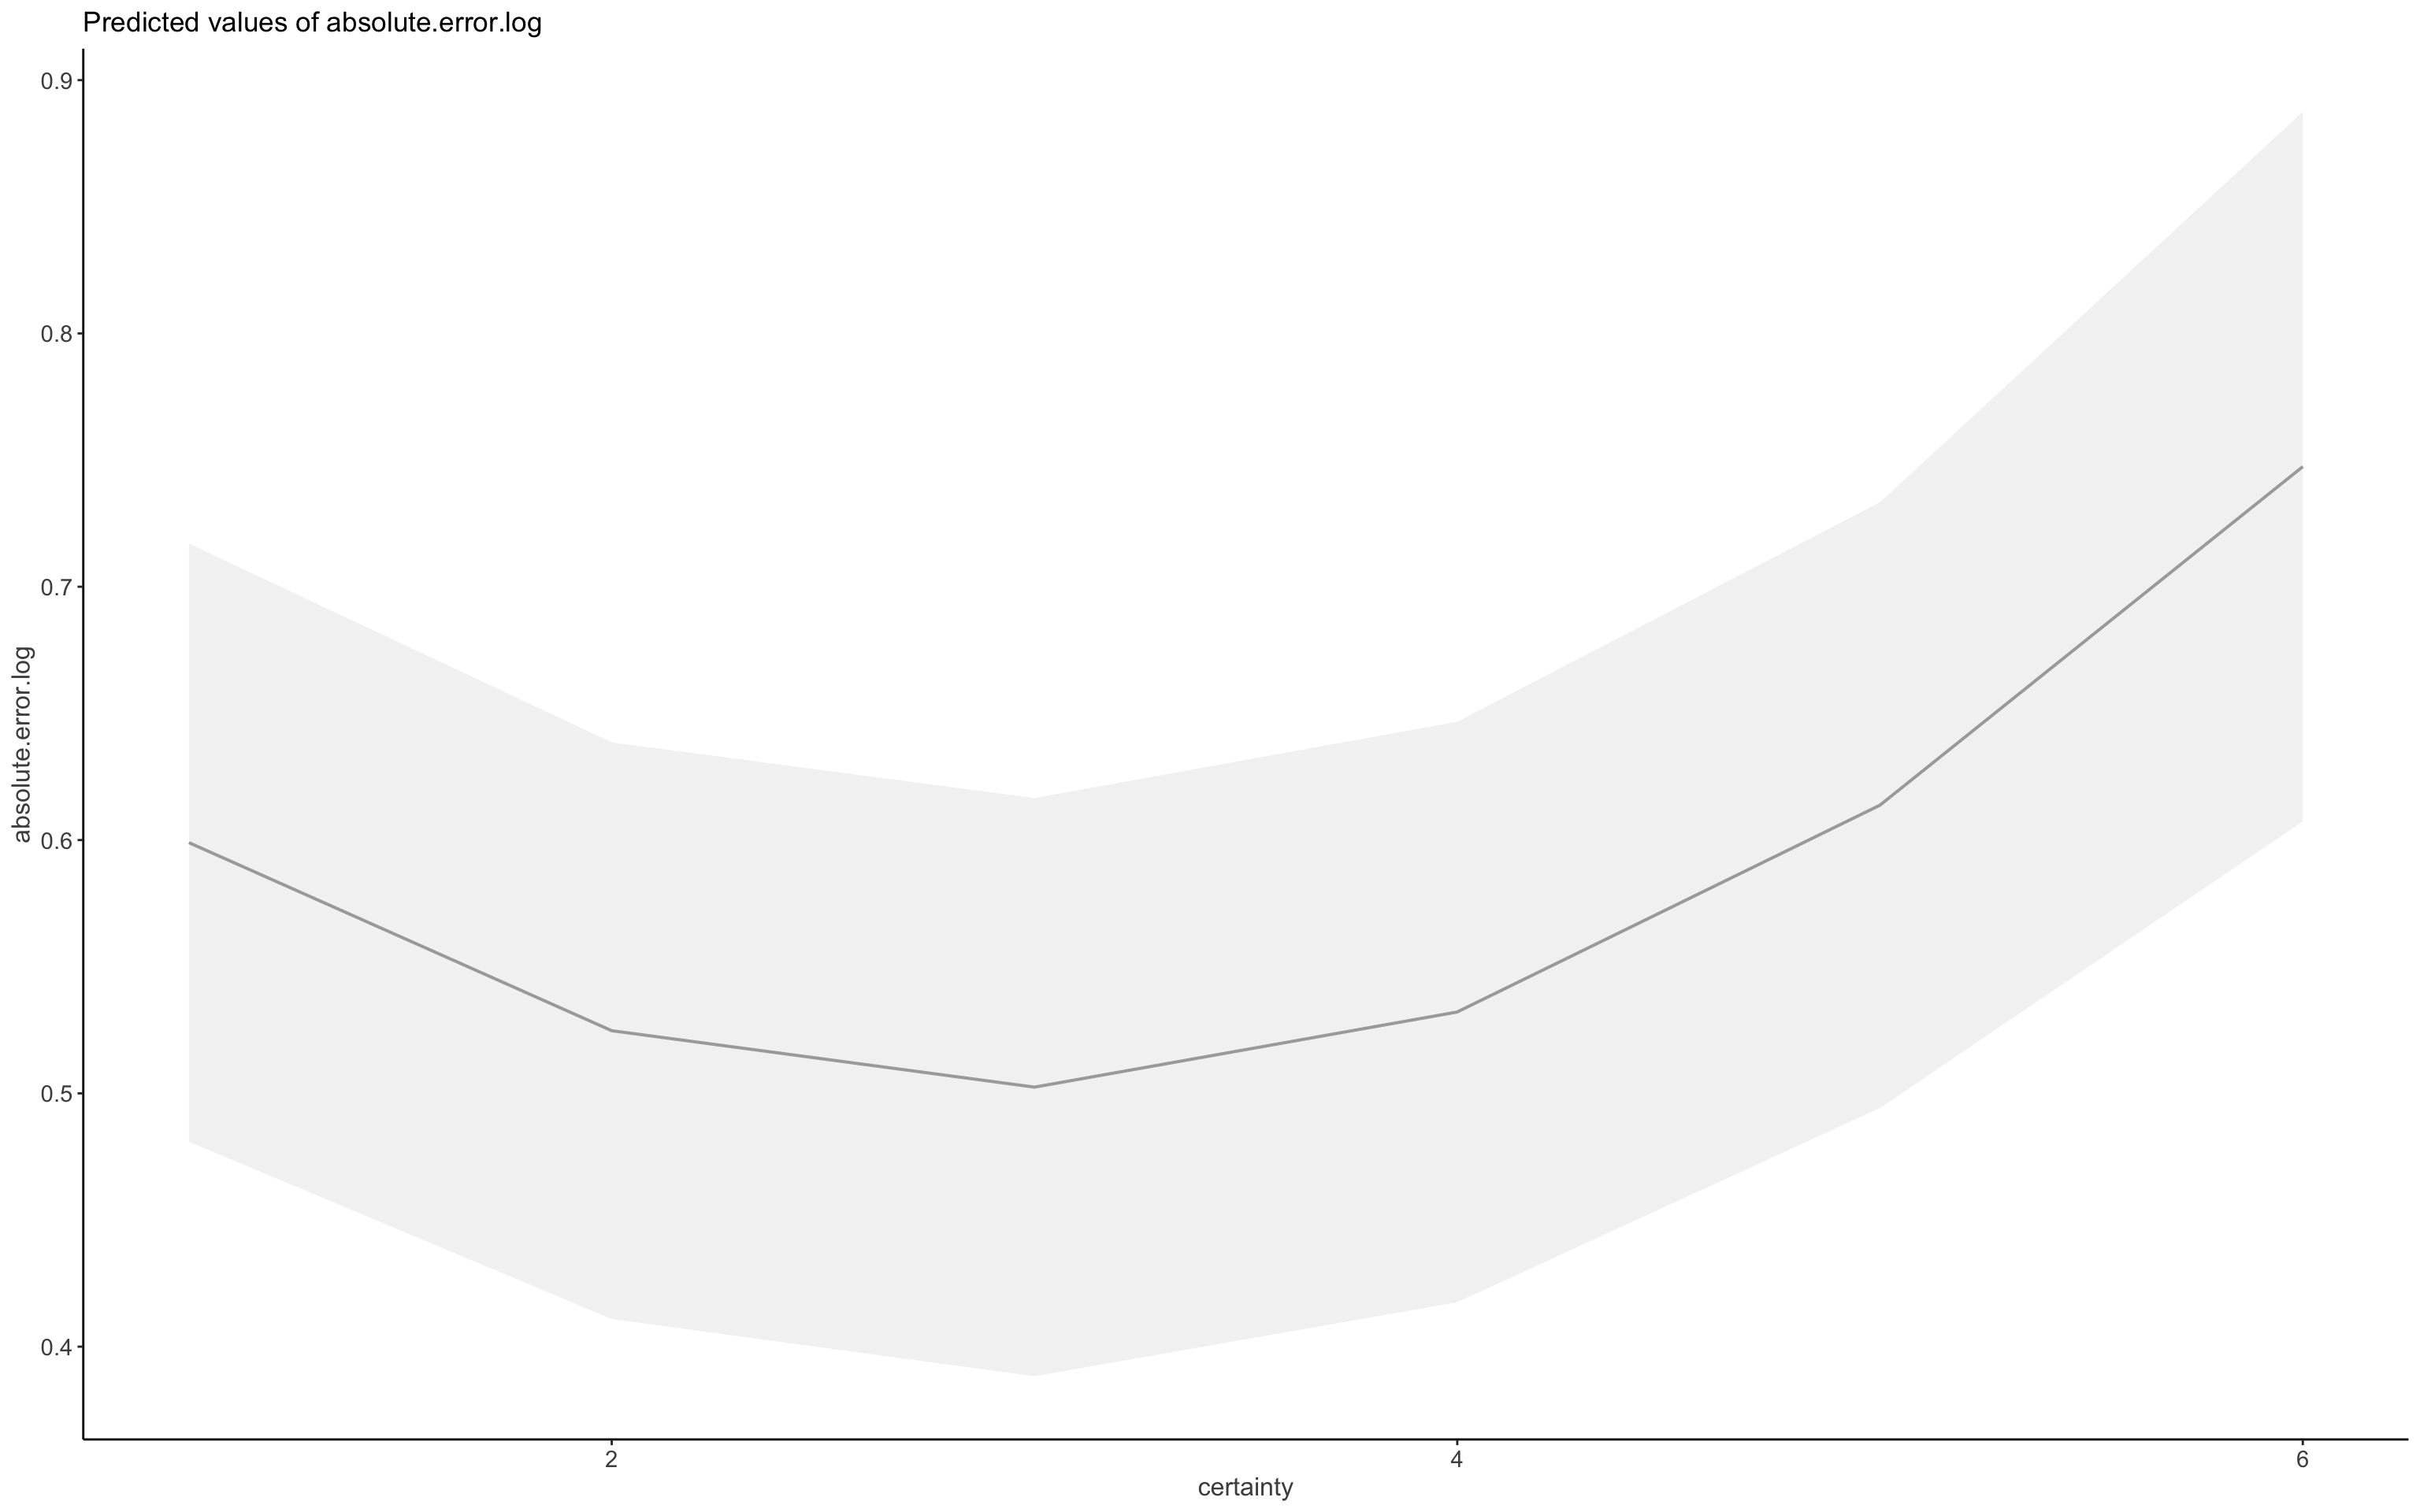
\includegraphics{analyses-judgment-new_files/figure-latex/unnamed-chunk-7-1} \end{center}

\hypertarget{h3b-cleaned}{%
\paragraph{H3b cleaned}\label{h3b-cleaned}}

Model with certainty and numeracy\\

~

absolute.error.log

Predictors

Estimates

CI

p

(Intercept)

0.65

0.55~--~0.76

\textless0.001

certainty

0.01

-0.00~--~0.02

0.099

numeracy f {[}numeracy low{]}

0.10

0.07~--~0.14

\textless0.001

education {[}middle school{]}

0.03

-0.01~--~0.07

0.180

education {[}no formaleducation{]}

0.07

0.02~--~0.13

0.014

education {[}obligatoryschool{]}

0.05

0.00~--~0.09

0.029

country \protect\hyperlink{switzerland}{Switzerland}

0.04

0.01~--~0.07

0.018

gender {[}male{]}

-0.04

-0.07~--~-0.00

0.023

income {[}\textless1'500€\textless3'100CHF{]}

0.03

-0.02~--~0.08

0.214

income {[}\textgreater{} 4'000€ \textgreater5'900CHF{]}

-0.00

-0.04~--~0.04

0.984

income {[}2'500- 4'000€\textless4'300- 5'899CHF{]}

0.02

-0.03~--~0.06

0.467

age

-0.00

-0.00~--~-0.00

\textless0.001

concern scaled

-0.02

-0.03~--~-0.01

\textless0.001

Random Effects

σ2

0.22

τ00 m

0.03

τ00 behavior

0.01

ICC

0.17

N m

980

N behavior

8

Observations

7840

Marginal R2 / Conditional R2

0.024 / 0.190

\hypertarget{h3b-plot-cleaned}{%
\paragraph{H3b plot (cleaned)}\label{h3b-plot-cleaned}}

\begin{center}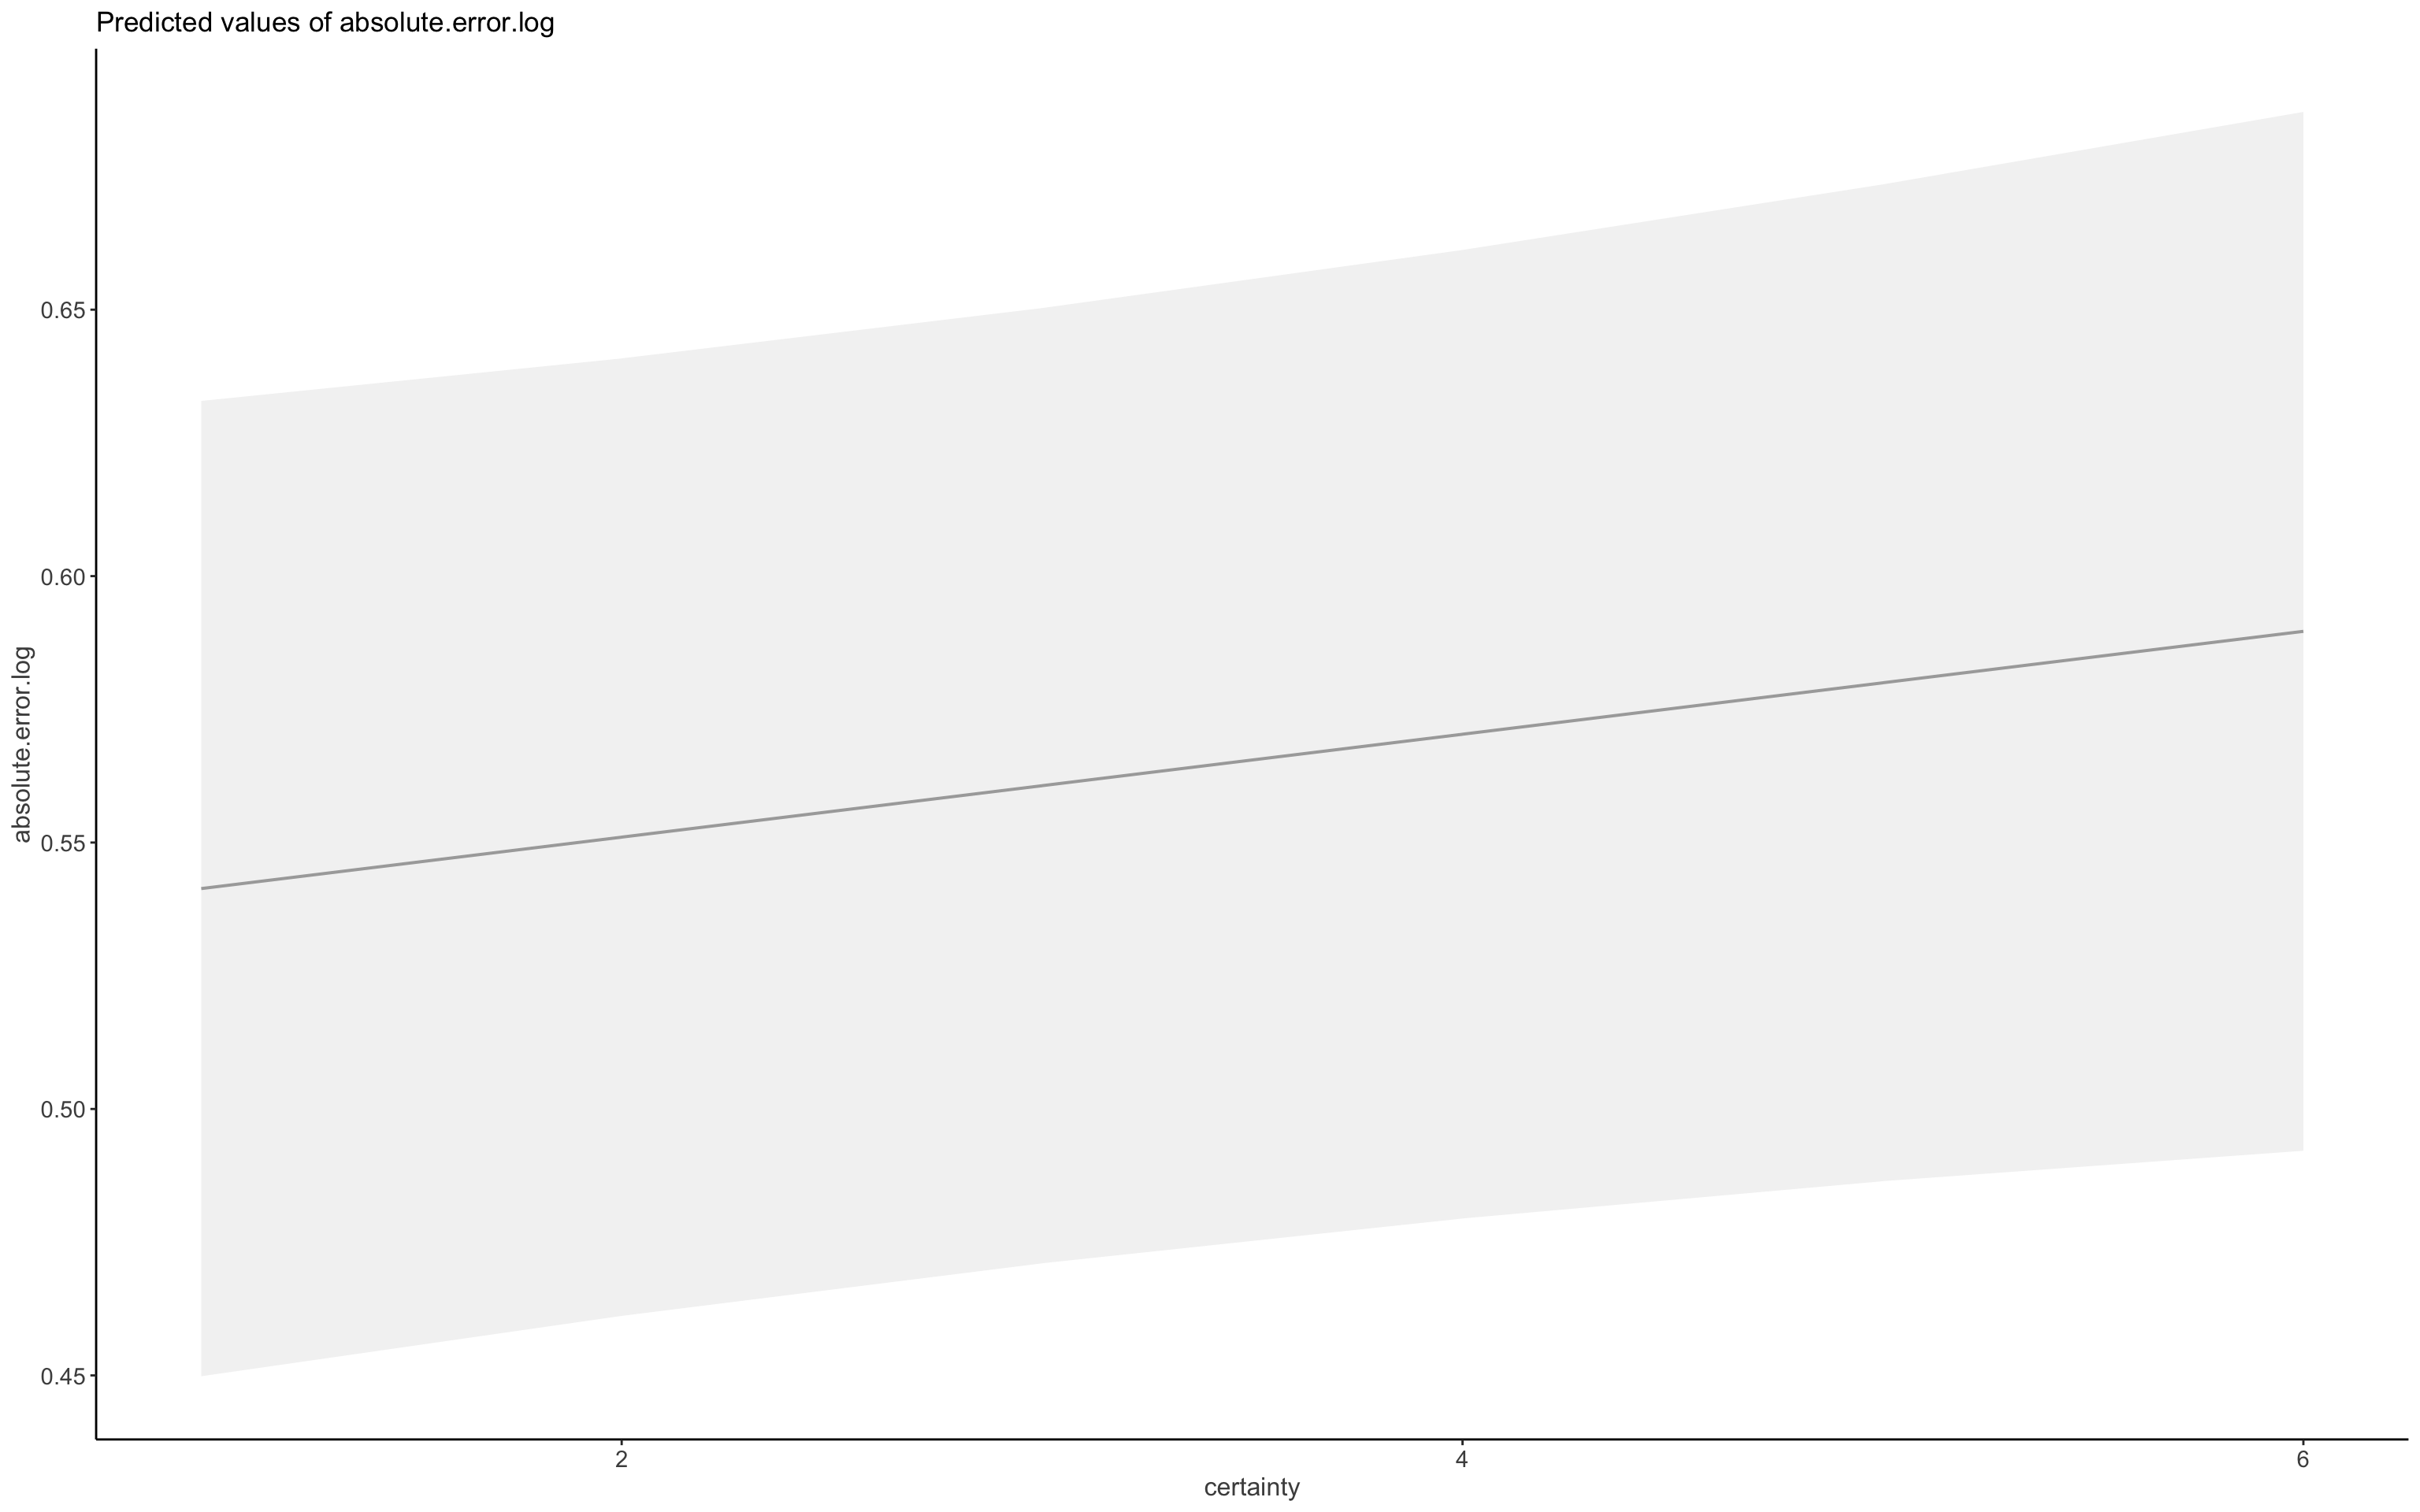
\includegraphics{analyses-judgment-new_files/figure-latex/unnamed-chunk-9-1} \end{center}

\hypertarget{h3b-cleaned-exponential}{%
\paragraph{H3b cleaned, exponential}\label{h3b-cleaned-exponential}}

~

absolute.error.log

Predictors

Estimates

CI

p

(Intercept)

0.78

0.66~--~0.90

\textless0.001

certainty

-0.10

-0.14~--~-0.05

\textless0.001

numeracy f {[}numeracy low{]}

0.10

0.06~--~0.14

\textless0.001

certainty\^{}2

0.02

0.01~--~0.02

\textless0.001

education {[}middle school{]}

0.03

-0.01~--~0.08

0.154

education {[}no formaleducation{]}

0.08

0.02~--~0.14

0.009

education {[}obligatoryschool{]}

0.05

0.01~--~0.09

0.023

country \protect\hyperlink{switzerland}{Switzerland}

0.04

0.01~--~0.07

0.016

gender {[}male{]}

-0.04

-0.07~--~-0.00

0.024

income {[}\textless1'500€\textless3'100CHF{]}

0.03

-0.02~--~0.08

0.174

income {[}\textgreater{} 4'000€ \textgreater5'900CHF{]}

0.00

-0.04~--~0.05

0.912

income {[}2'500- 4'000€\textless4'300- 5'899CHF{]}

0.02

-0.02~--~0.06

0.409

age

-0.00

-0.00~--~-0.00

\textless0.001

concern scaled

-0.02

-0.03~--~-0.01

\textless0.001

Random Effects

σ2

0.22

τ00 m

0.03

τ00 behavior

0.01

ICC

0.17

N m

980

N behavior

8

Observations

7840

Marginal R2 / Conditional R2

0.028 / 0.192

\hypertarget{h3b-cleaned-exponential-plot}{%
\paragraph{H3b (cleaned) exponential
plot}\label{h3b-cleaned-exponential-plot}}

\begin{verbatim}
## Model contains polynomial or cubic / quadratic terms. Consider using
##   `terms="certainty [all]"` to get smooth plots. See also package-vignette
##   'Marginal Effects at Specific Values'.
\end{verbatim}

\begin{center}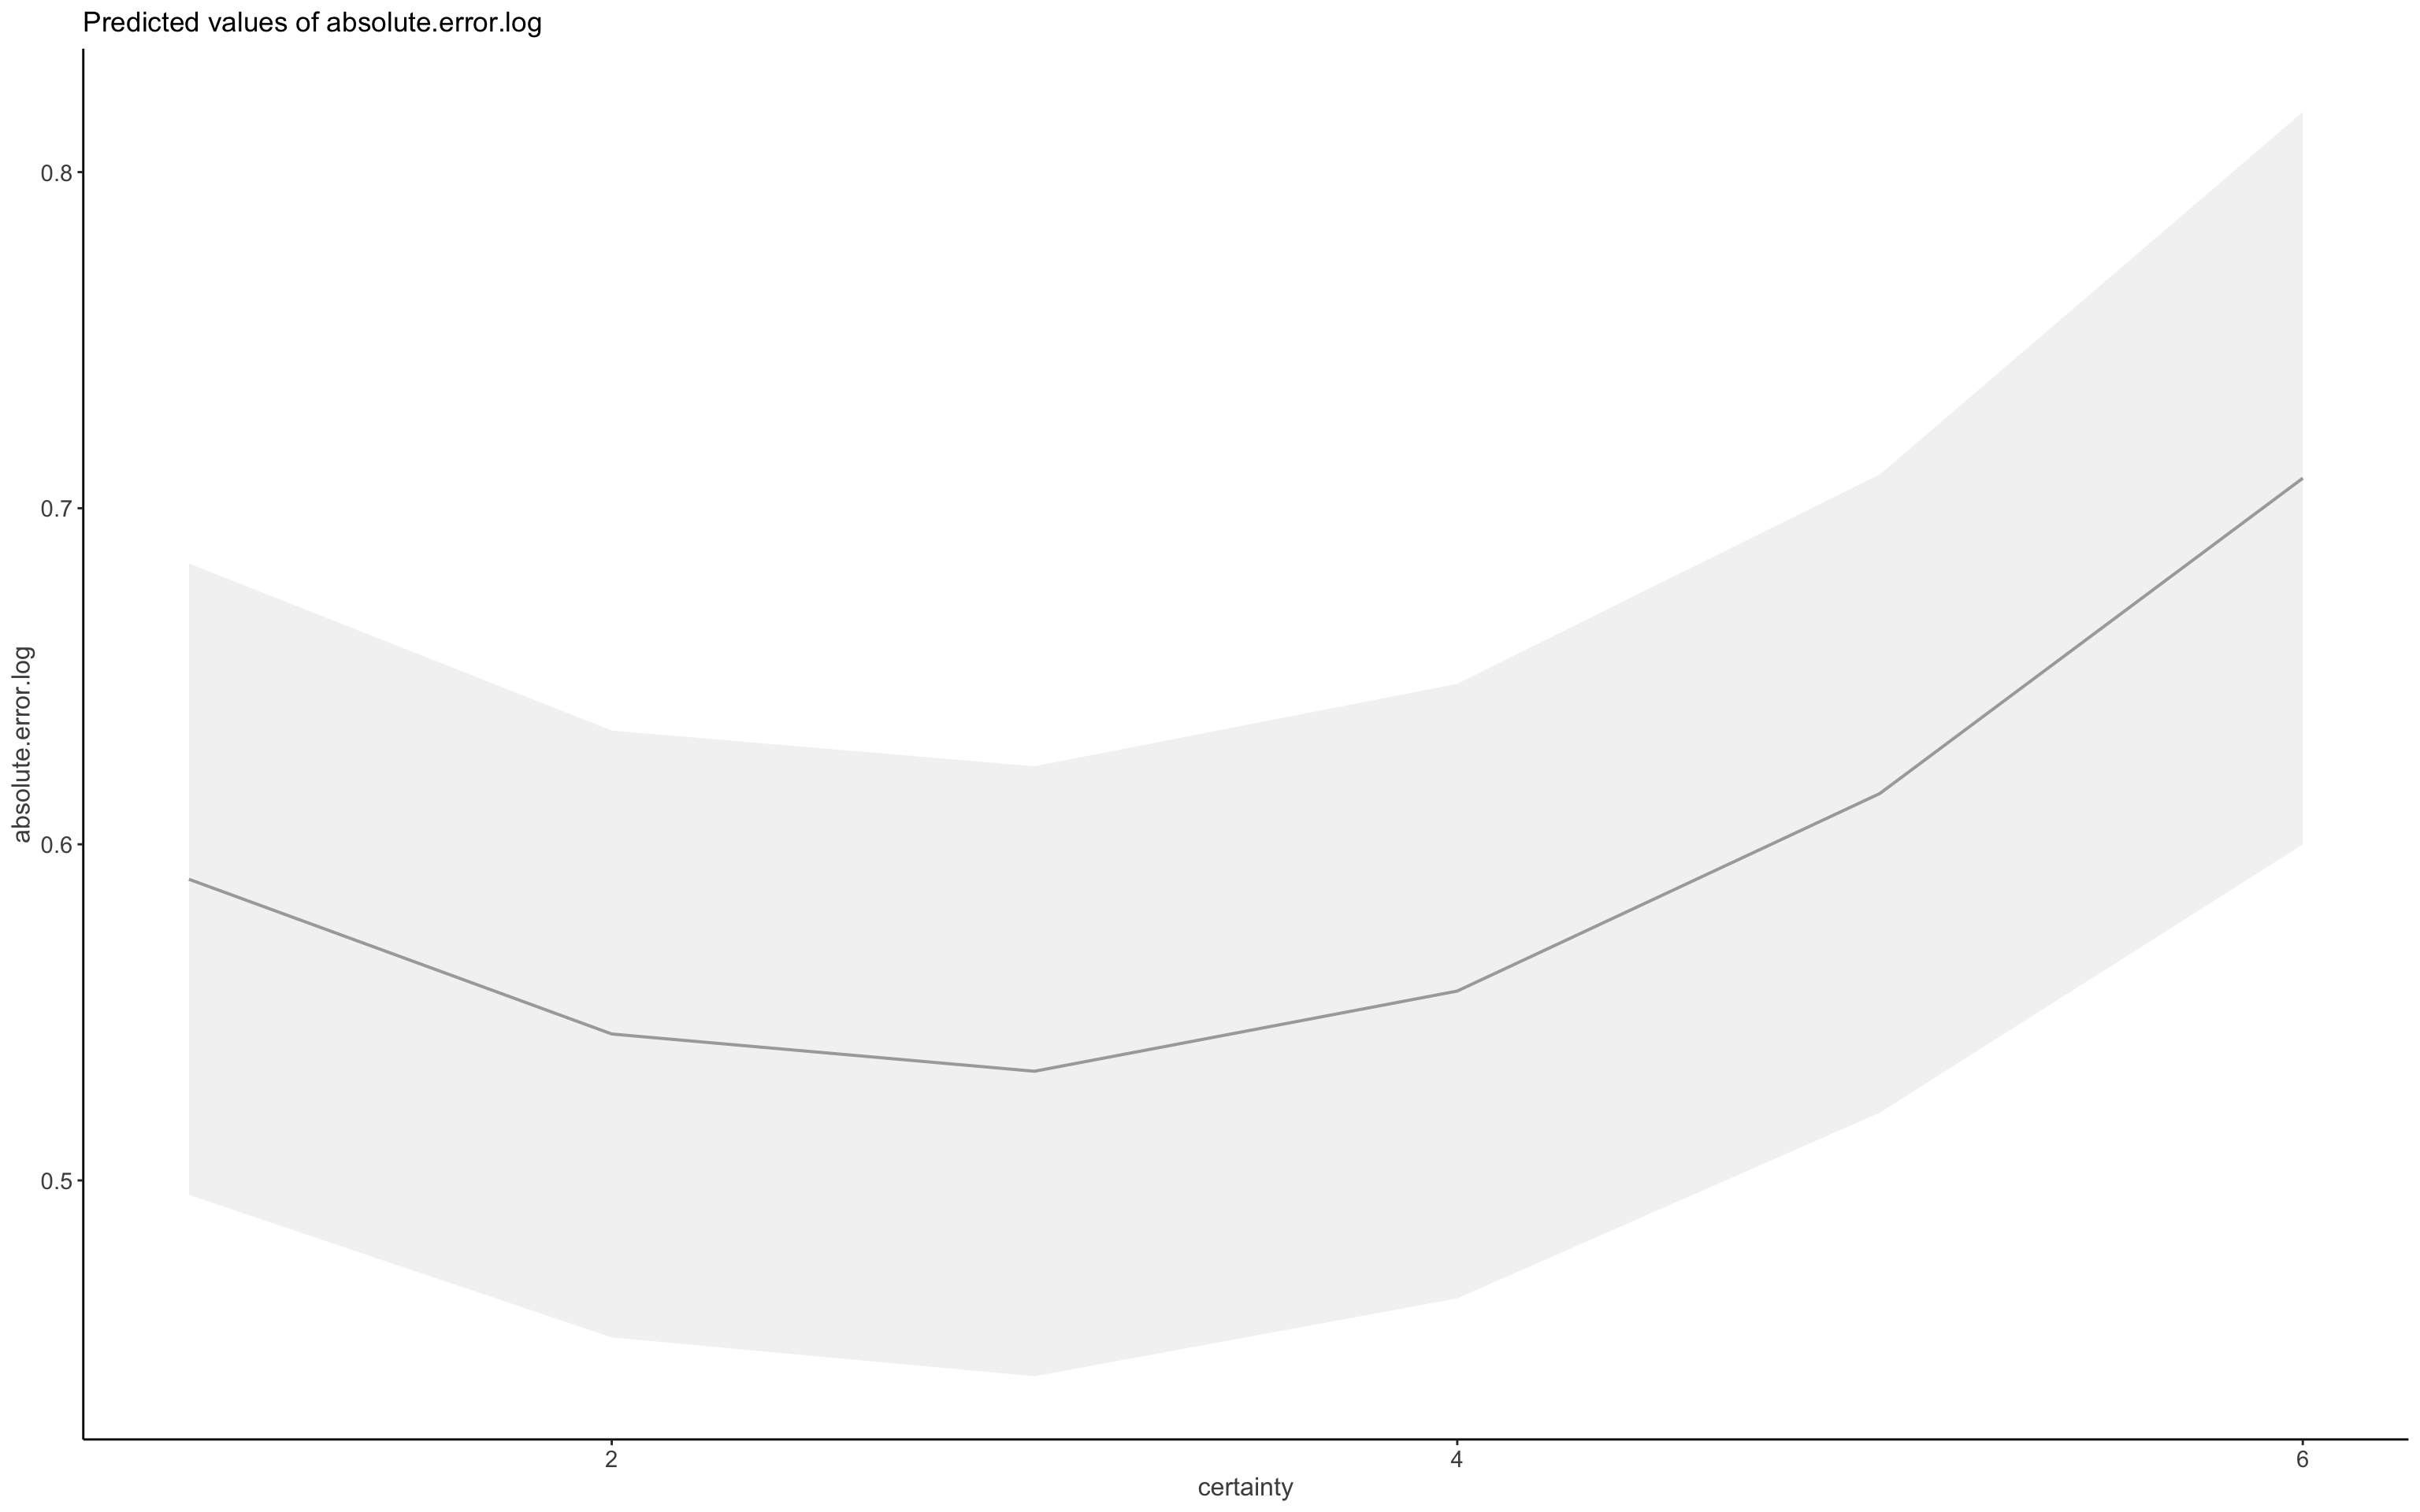
\includegraphics{analyses-judgment-new_files/figure-latex/unnamed-chunk-11-1} \end{center}

\hypertarget{judgment-estimates-and-actual-values-both-waves-together}{%
\subsection{Judgment estimates and actual values both waves
together}\label{judgment-estimates-and-actual-values-both-waves-together}}

\hypertarget{cleaned-for-pattern-people-fig-2a}{%
\subsubsection{cleaned for pattern people Fig
2a}\label{cleaned-for-pattern-people-fig-2a}}

\begin{center}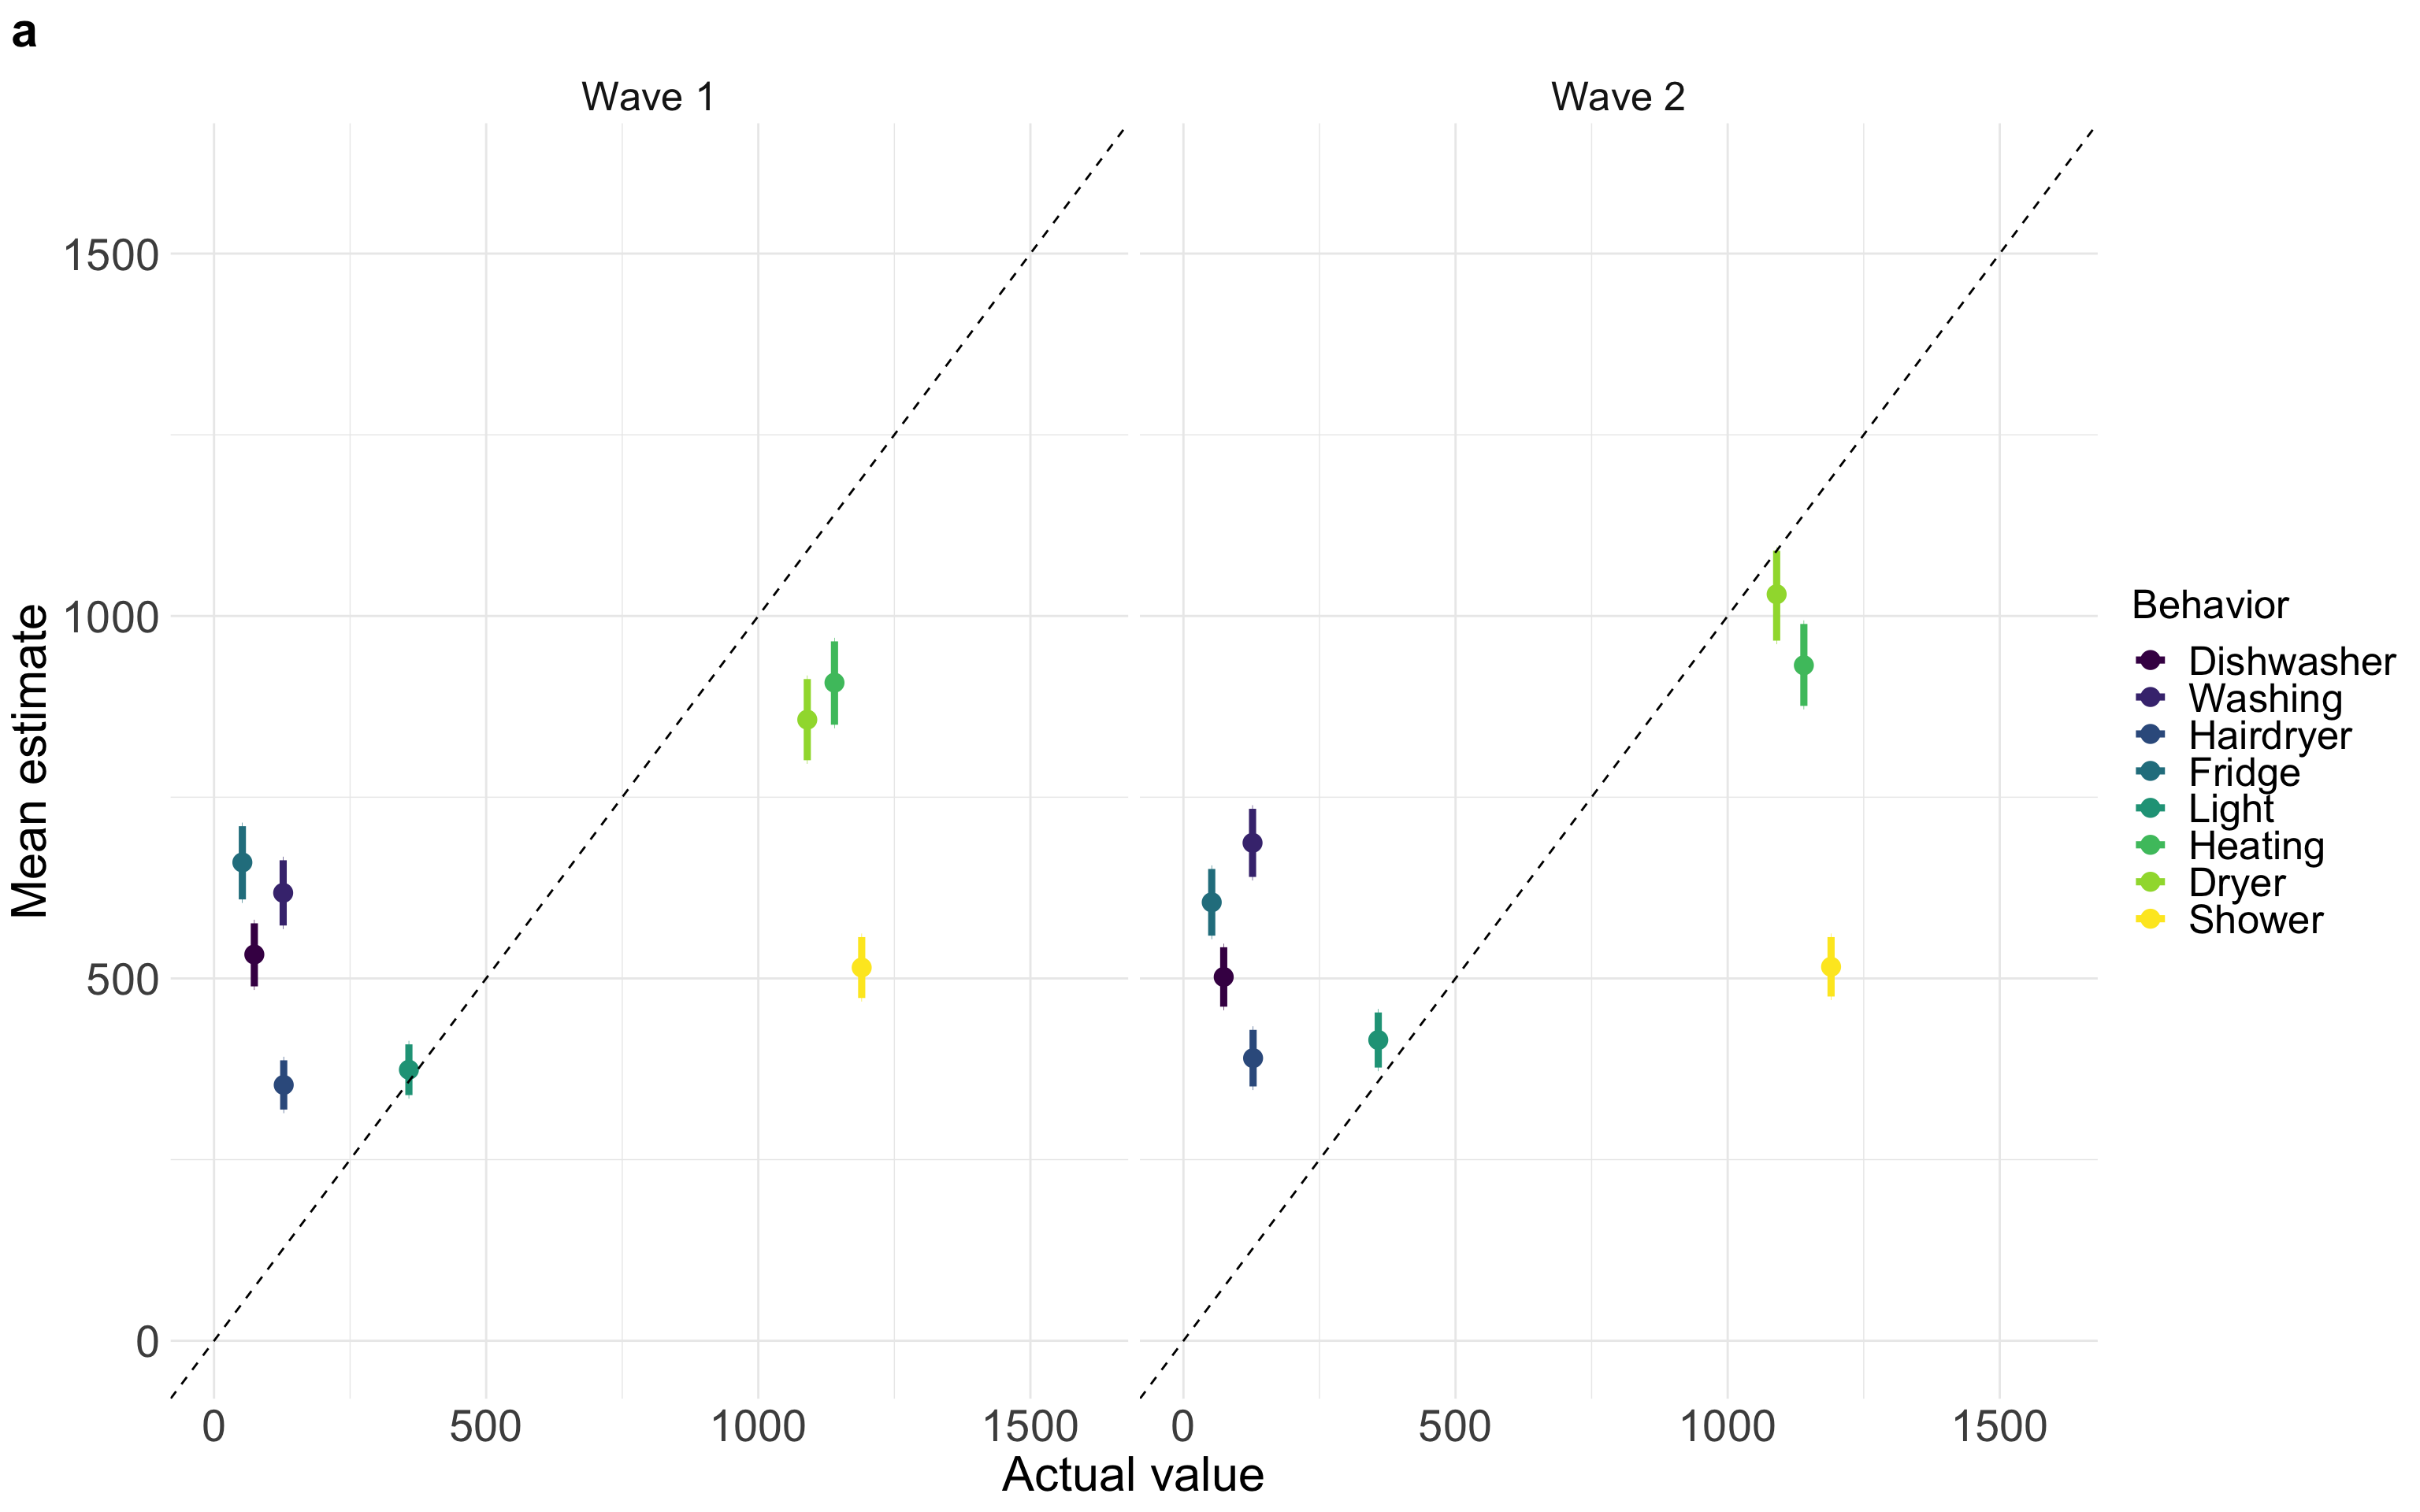
\includegraphics{analyses-judgment-new_files/figure-latex/unnamed-chunk-13-1} \end{center}

\hypertarget{misestimation-of-impact-across-waves}{%
\subsection{misestimation of impact across
waves}\label{misestimation-of-impact-across-waves}}

\hypertarget{not-cleaned}{%
\subsubsection{not cleaned}\label{not-cleaned}}

\begin{verbatim}
##   impact  wave    n  Mean Conf.level Trad.lower Trad.upper    Mean.2
## 1   high wave1 3108 0.649       0.95      0.623      0.676 1.5408320
## 2   high wave2 3108 0.722       0.95      0.694      0.750 1.3850416
## 3    low wave1 5180 5.550       0.95      5.290      5.800 0.1801802
## 4    low wave2 5180 5.590       0.95      5.340      5.840 0.1788909
##   Trad.lower2 Trad.upper2
## 1   1.6051364   1.4792899
## 2   1.4409222   1.3333333
## 3   0.1890359   0.1724138
## 4   0.1872659   0.1712329
\end{verbatim}

\begin{verbatim}
## 
##  Paired t-test
## 
## data:  data.accuracy.waves.long.total2.l$mis.estimation by data.accuracy.waves.long.total2.l$wave
## t = -0.62413, df = 8287, p-value = 0.5326
## alternative hypothesis: true mean difference is not equal to 0
## 95 percent confidence interval:
##  -0.2302919  0.1190601
## sample estimates:
## mean difference 
##     -0.05561587
\end{verbatim}

\begin{verbatim}
## ANOVA Table (type III tests)
## 
##        Effect DFn  DFd        F         p p<.05      ges
## 1        wave   1 1035    0.249  6.18e-01       4.75e-05
## 2      impact   1 1035 1215.529 8.96e-177     * 2.44e-01
## 3 wave:impact   1 1035    0.018  8.95e-01       2.46e-06
\end{verbatim}

\hypertarget{cleaned}{%
\subsubsection{cleaned}\label{cleaned}}

\begin{verbatim}
##   impact  wave    n  Mean Conf.level Trad.lower Trad.upper    Mean.2
## 1   high wave1 2940 0.672       0.95      0.645       0.70 1.4880952
## 2   high wave2 2940 0.732       0.95      0.703       0.76 1.3661202
## 3    low wave1 4900 5.710       0.95      5.440       5.98 0.1751313
## 4    low wave2 4900 5.610       0.95      5.360       5.86 0.1782531
##   Trad.lower2 Trad.upper2
## 1   1.5503876   1.4285714
## 2   1.4224751   1.3157895
## 3   0.1838235   0.1672241
## 4   0.1865672   0.1706485
\end{verbatim}

\begin{verbatim}
## 
##  Paired t-test
## 
## data:  data.accuracy.waves.long.total_clean2$mis.estimation by data.accuracy.waves.long.total_clean2$wave
## t = 0.46993, df = 7839, p-value = 0.6384
## alternative hypothesis: true mean difference is not equal to 0
## 95 percent confidence interval:
##  -0.1344126  0.2191787
## sample estimates:
## mean difference 
##      0.04238306
\end{verbatim}

\begin{verbatim}
## ANOVA Table (type III tests)
## 
##        Effect DFn DFd        F        p p<.05      ges
## 1        wave   1 979    0.192 6.62e-01       6.19e-05
## 2      impact   1 979 7624.582 0.00e+00     * 2.83e-01
## 3 wave:impact   1 979   16.174 6.22e-05     * 4.01e-04
\end{verbatim}

\begin{verbatim}
## Analysis of Deviance Table (Type III Wald F tests with Kenward-Roger df)
## 
## Response: Mean
##                     F Df Df.res  Pr(>F)    
## (Intercept)  125.7957  1    979 < 2e-16 ***
## impact      2967.6195  1   2937 < 2e-16 ***
## wave           0.4645  1   2937 0.49559    
## impact:wave    3.0118  1   2937 0.08277 .  
## ---
## Signif. codes:  0 '***' 0.001 '**' 0.01 '*' 0.05 '.' 0.1 ' ' 1
\end{verbatim}

\hypertarget{mean-judgment-error-across-waves-by-numeracy}{%
\subsection{Mean judgment error across waves by
numeracy}\label{mean-judgment-error-across-waves-by-numeracy}}

\hypertarget{witout-pattern-people-fig-2b}{%
\subsubsection{witout pattern people fig
2b}\label{witout-pattern-people-fig-2b}}

\begin{center}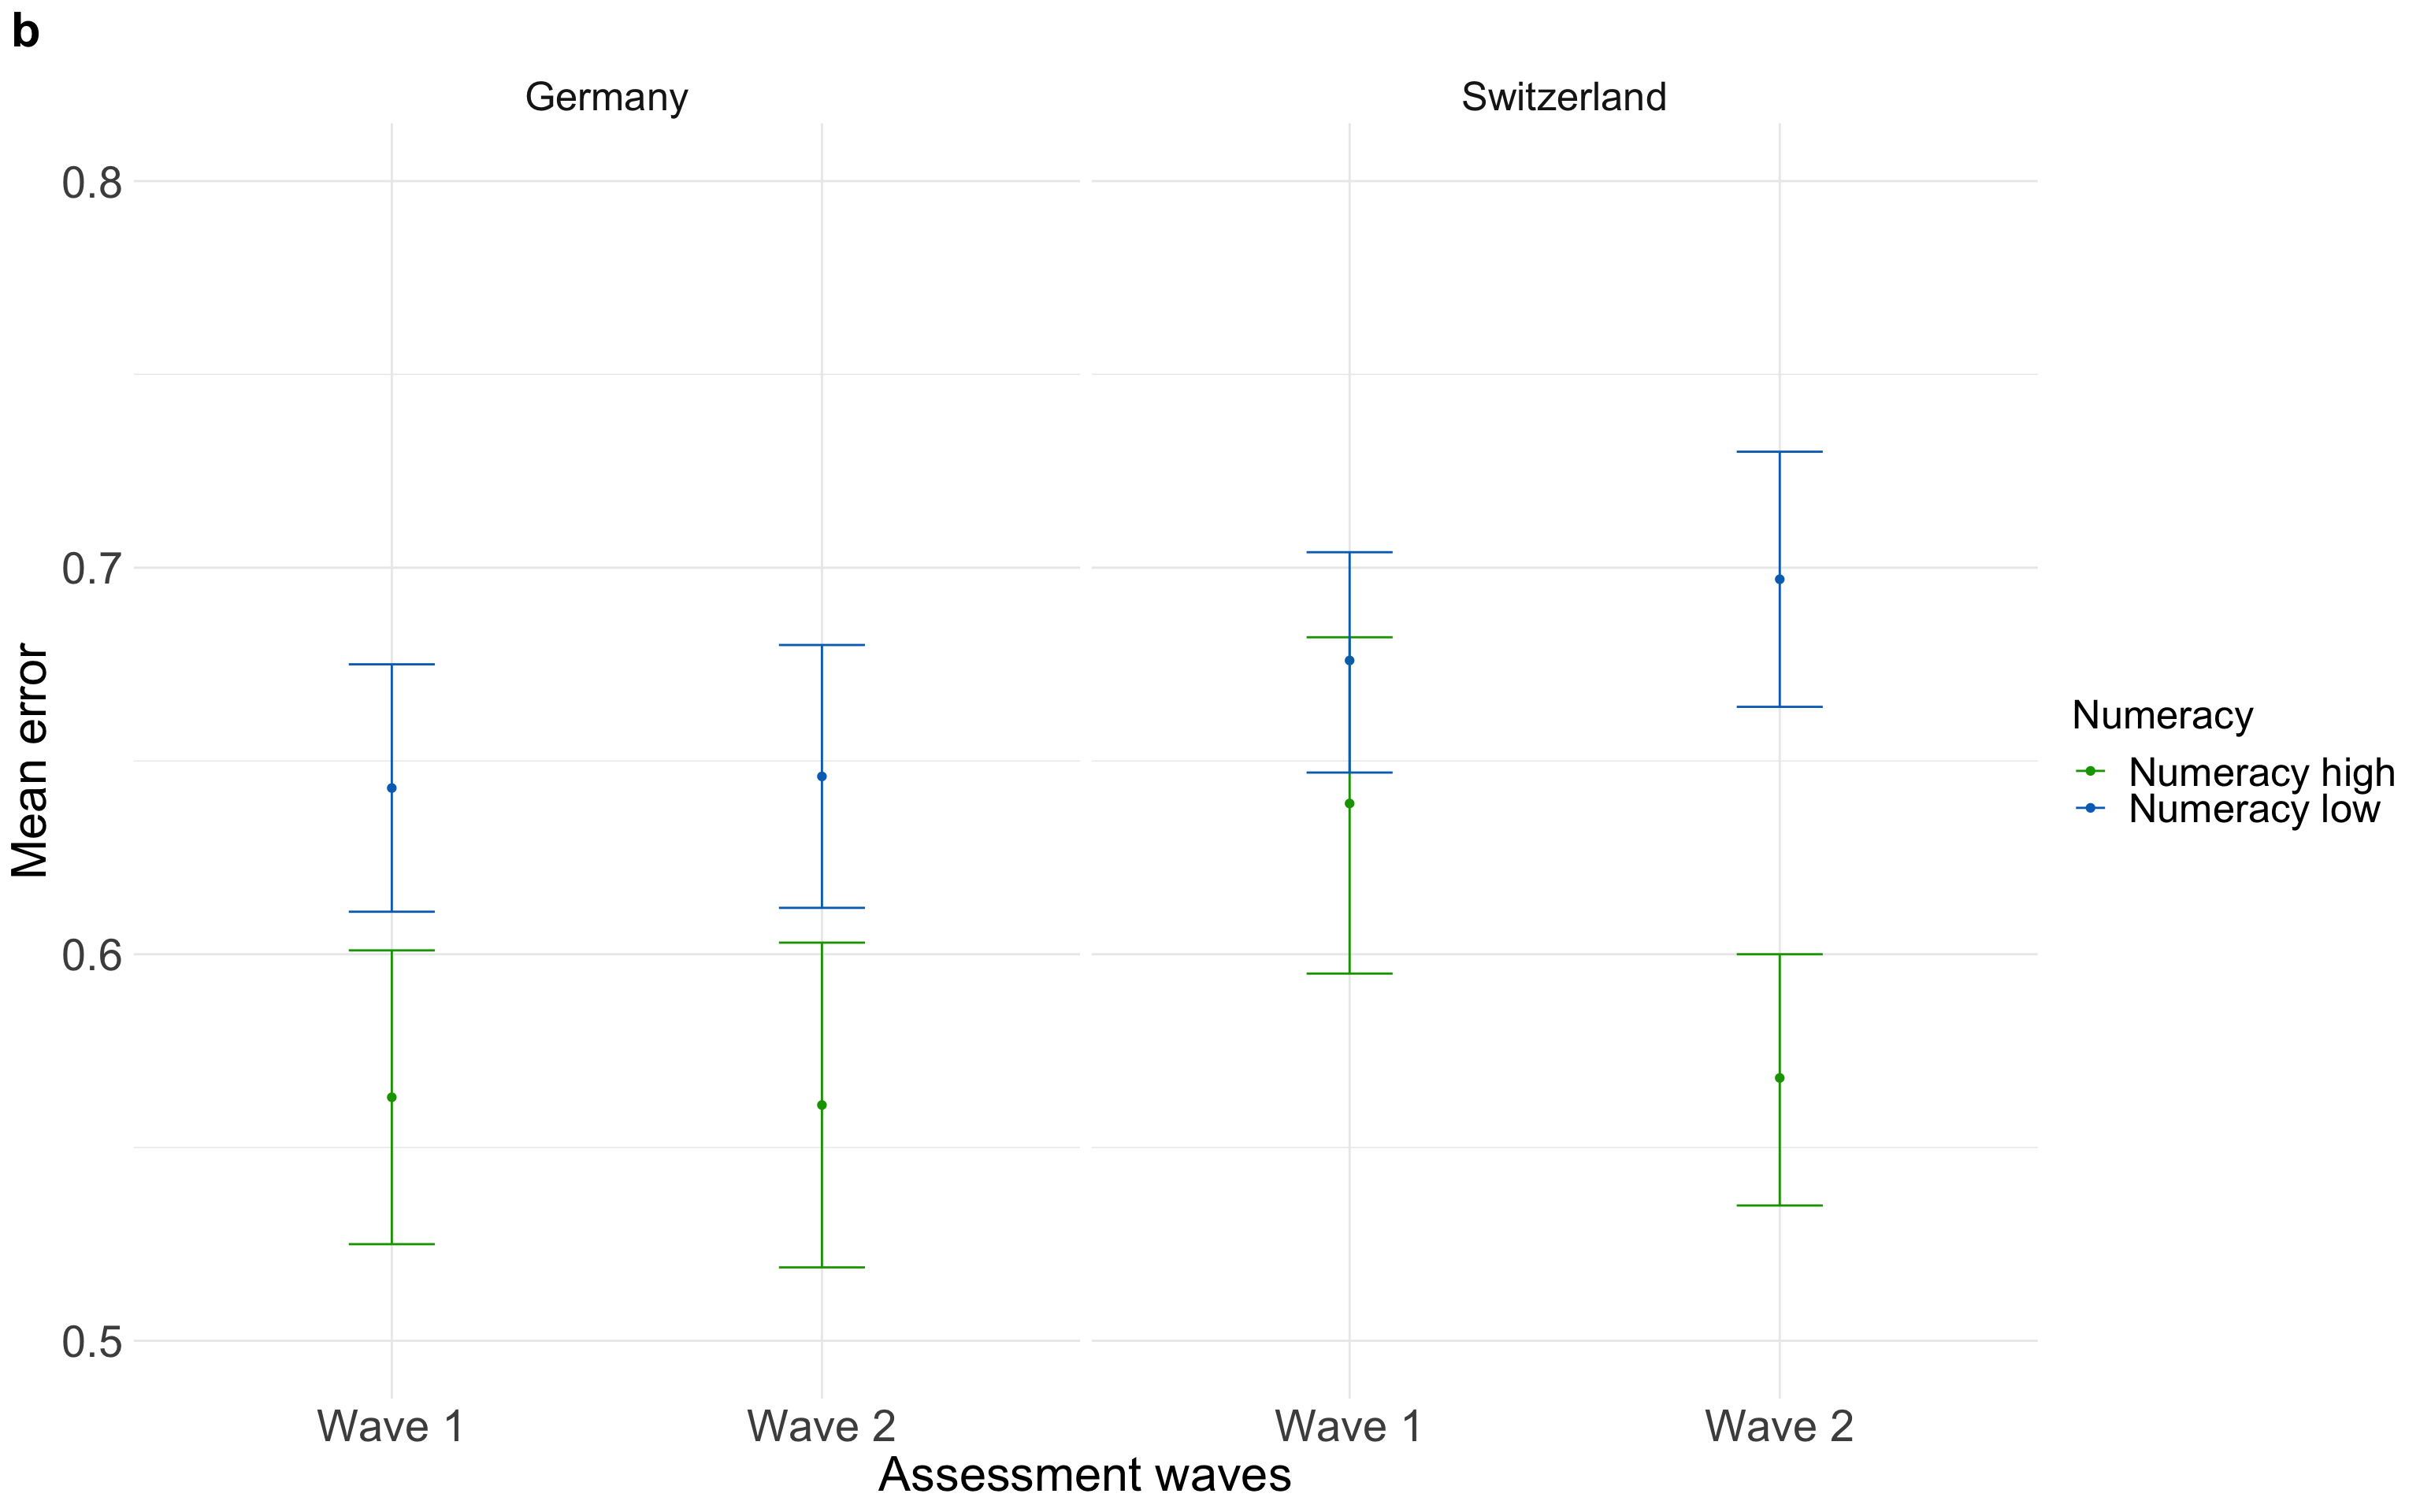
\includegraphics{analyses-judgment-new_files/figure-latex/unnamed-chunk-19-1} \end{center}

Both judgment figures

\begin{center}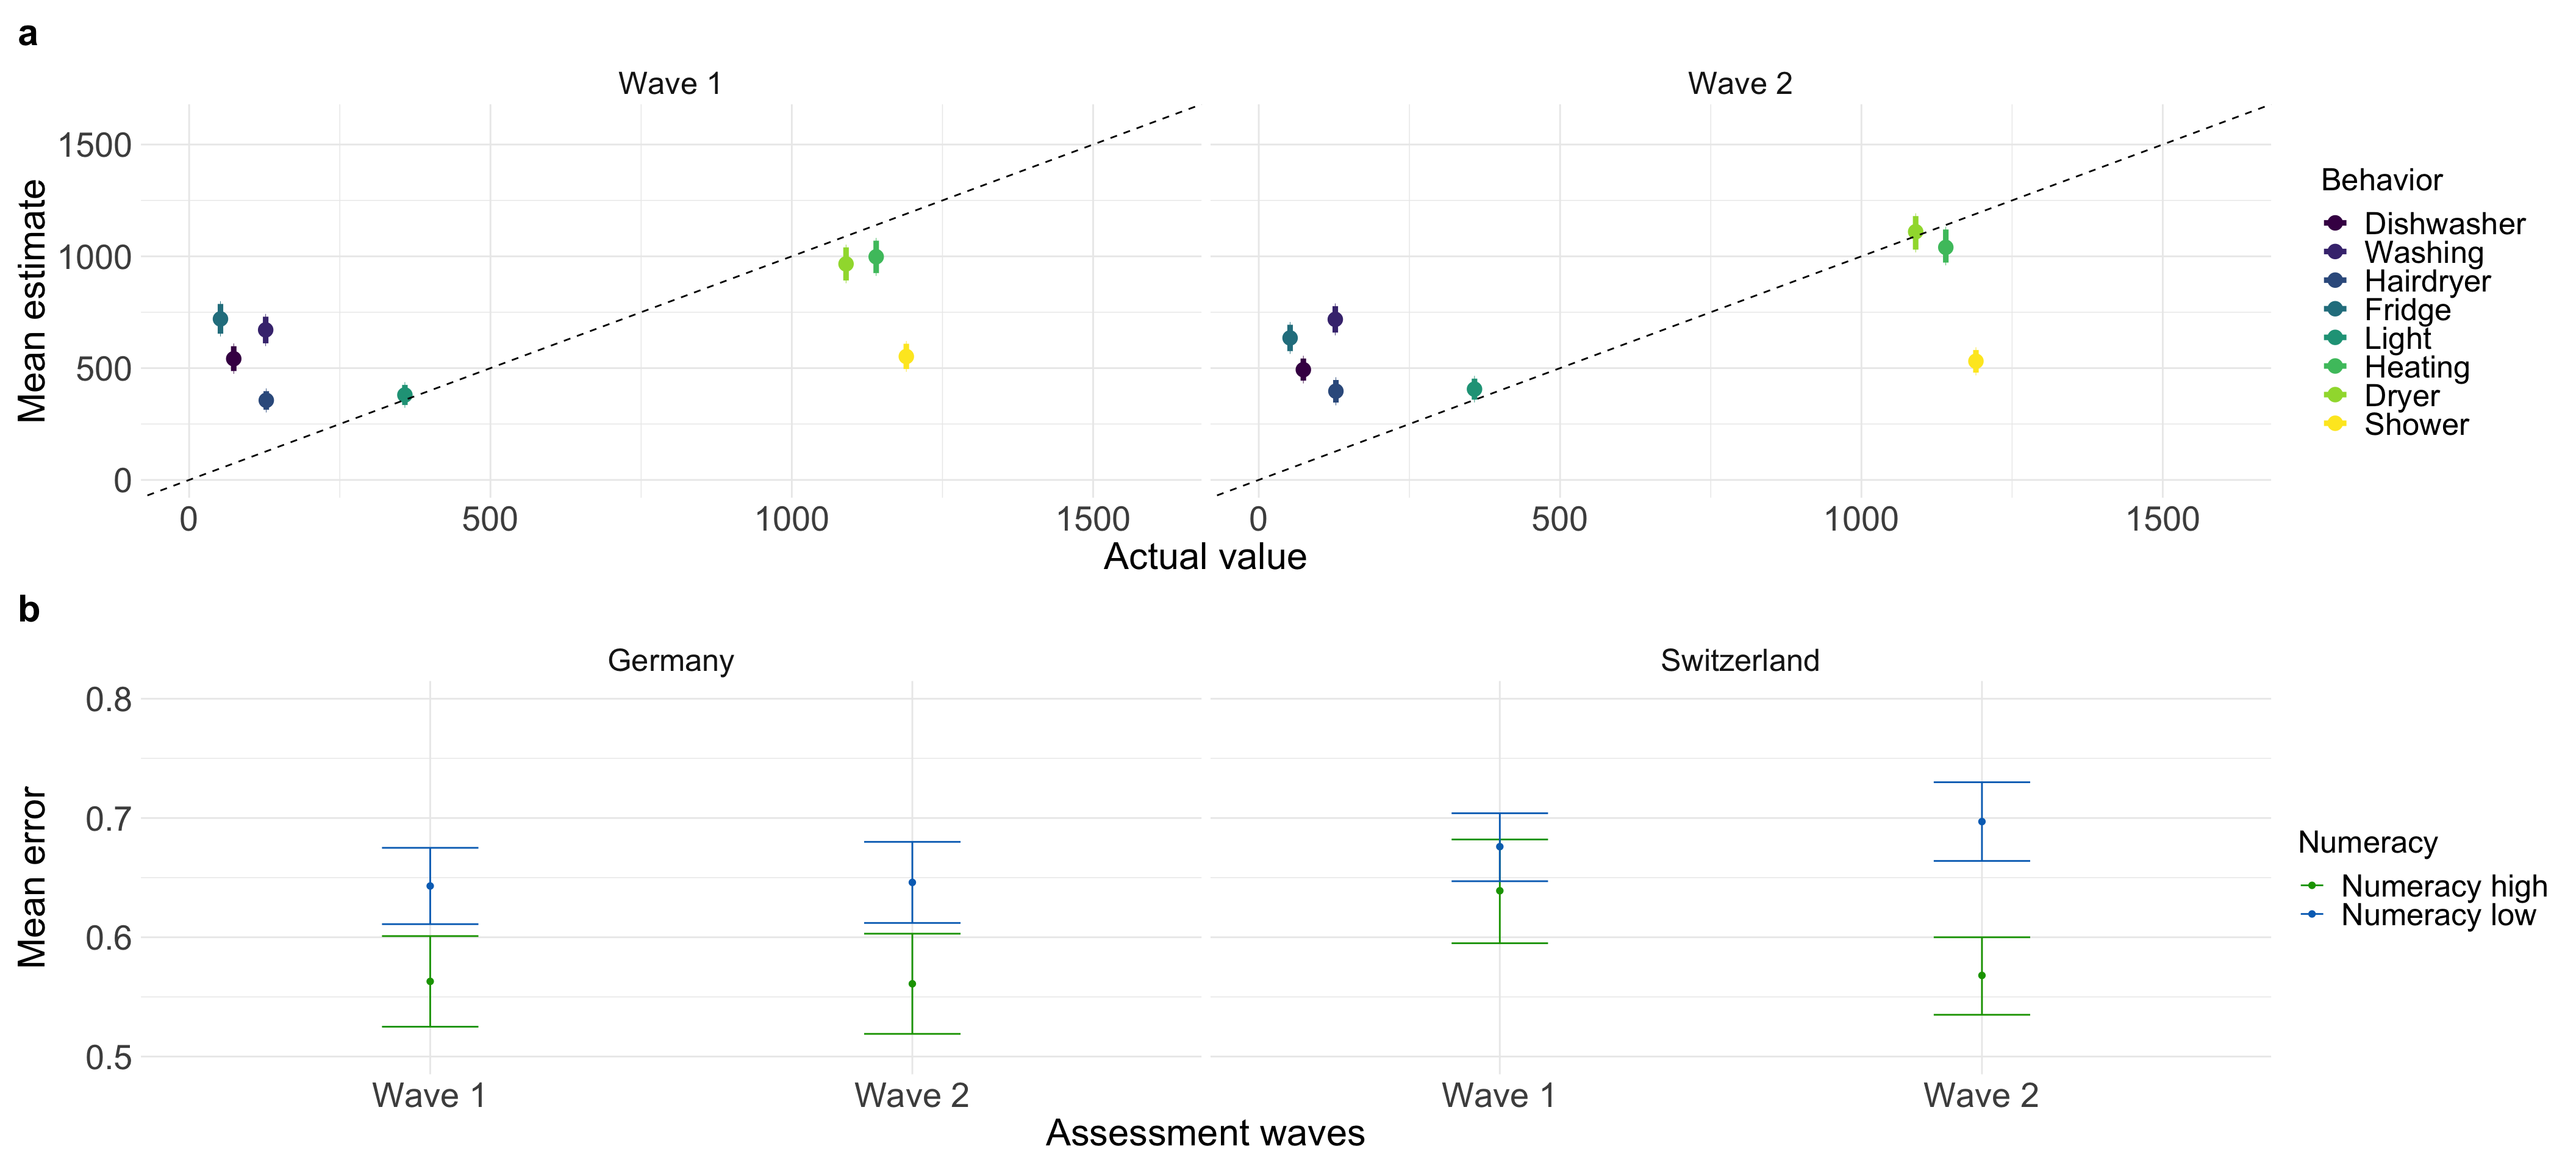
\includegraphics{analyses-judgment-new_files/figure-latex/unnamed-chunk-20-1} \end{center}

\hypertarget{across-waves-judgment-error}{%
\subsection{Across waves judgment
error}\label{across-waves-judgment-error}}

same approach as misestimation for judgment error

Models cleaned for pattern people

\begin{verbatim}
##      numeracy.f  wave    n  Mean Conf.level Trad.lower Trad.upper   Mean.2
## 1 numeracy high wave1 1800 0.617       0.95      0.594      0.639 1.620746
## 2 numeracy high wave2 1800 0.592       0.95      0.570      0.613 1.689189
## 3  numeracy low wave1 6040 0.690       0.95      0.677      0.702 1.449275
## 4  numeracy low wave2 6040 0.710       0.95      0.697      0.724 1.408451
##   Trad.lower2 Trad.upper2
## 1    1.683502    1.564945
## 2    1.754386    1.631321
## 3    1.477105    1.424501
## 4    1.434720    1.381215
\end{verbatim}

\begin{verbatim}
## 
##  Paired t-test
## 
## data:  accuracy.waves.error.num$Mean by accuracy.waves.error.num$wave
## t = -0.44352, df = 1959, p-value = 0.6574
## alternative hypothesis: true mean difference is not equal to 0
## 95 percent confidence interval:
##  -0.02606782  0.01645201
## sample estimates:
## mean difference 
##    -0.004807908
\end{verbatim}

\begin{verbatim}
## Analysis of Deviance Table (Type III Wald F tests with Kenward-Roger df)
## 
## Response: error
##                         F Df  Df.res    Pr(>F)    
## (Intercept)     7296.7998  1  1011.3 < 2.2e-16 ***
## numeracy.f        41.0589  1   977.0 2.294e-10 ***
## wave               0.6490  1 14696.0  0.420482    
## impact             4.4170  1 14696.0  0.035601 *  
## country            6.4215  1   977.0  0.011430 *  
## numeracy.f:wave    6.2639  1 14696.0  0.012333 *  
## wave:impact        7.1343  1 14696.0  0.007571 ** 
## ---
## Signif. codes:  0 '***' 0.001 '**' 0.01 '*' 0.05 '.' 0.1 ' ' 1
\end{verbatim}

\begin{verbatim}
## # Effect Size for ANOVA (Type III)
## 
## Parameter       | Eta2 (partial) |       95% CI
## -----------------------------------------------
## numeracy.f      |           0.04 | [0.02, 1.00]
## wave            |       4.42e-05 | [0.00, 1.00]
## impact          |       3.00e-04 | [0.00, 1.00]
## country         |       6.53e-03 | [0.00, 1.00]
## numeracy.f:wave |       4.26e-04 | [0.00, 1.00]
## wave:impact     |       4.85e-04 | [0.00, 1.00]
## 
## - One-sided CIs: upper bound fixed at [1.00].
\end{verbatim}

~

error

Predictors

Estimates

CI

p

(Intercept)

0.65

0.64~--~0.67

\textless0.001

numeracy f1

-0.05

-0.06~--~-0.03

\textless0.001

wave1

0.00

-0.01~--~0.01

0.420

impact1

0.01

0.00~--~0.02

0.036

country1

-0.02

-0.03~--~-0.00

0.011

numeracy f1 × wave1

0.01

0.00~--~0.02

0.012

wave1 × impact1

-0.01

-0.02~--~-0.00

0.008

Random Effects

σ2

0.23

τ00 m

0.02

ICC

0.10

N m

980

Observations

15680

Marginal R2 / Conditional R2

0.008 / 0.104

\hypertarget{plots-judgment-error-for-impact-of-actions-across-waves}{%
\subsubsection{Plots: Judgment error for impact of actions across
waves}\label{plots-judgment-error-for-impact-of-actions-across-waves}}

\begin{center}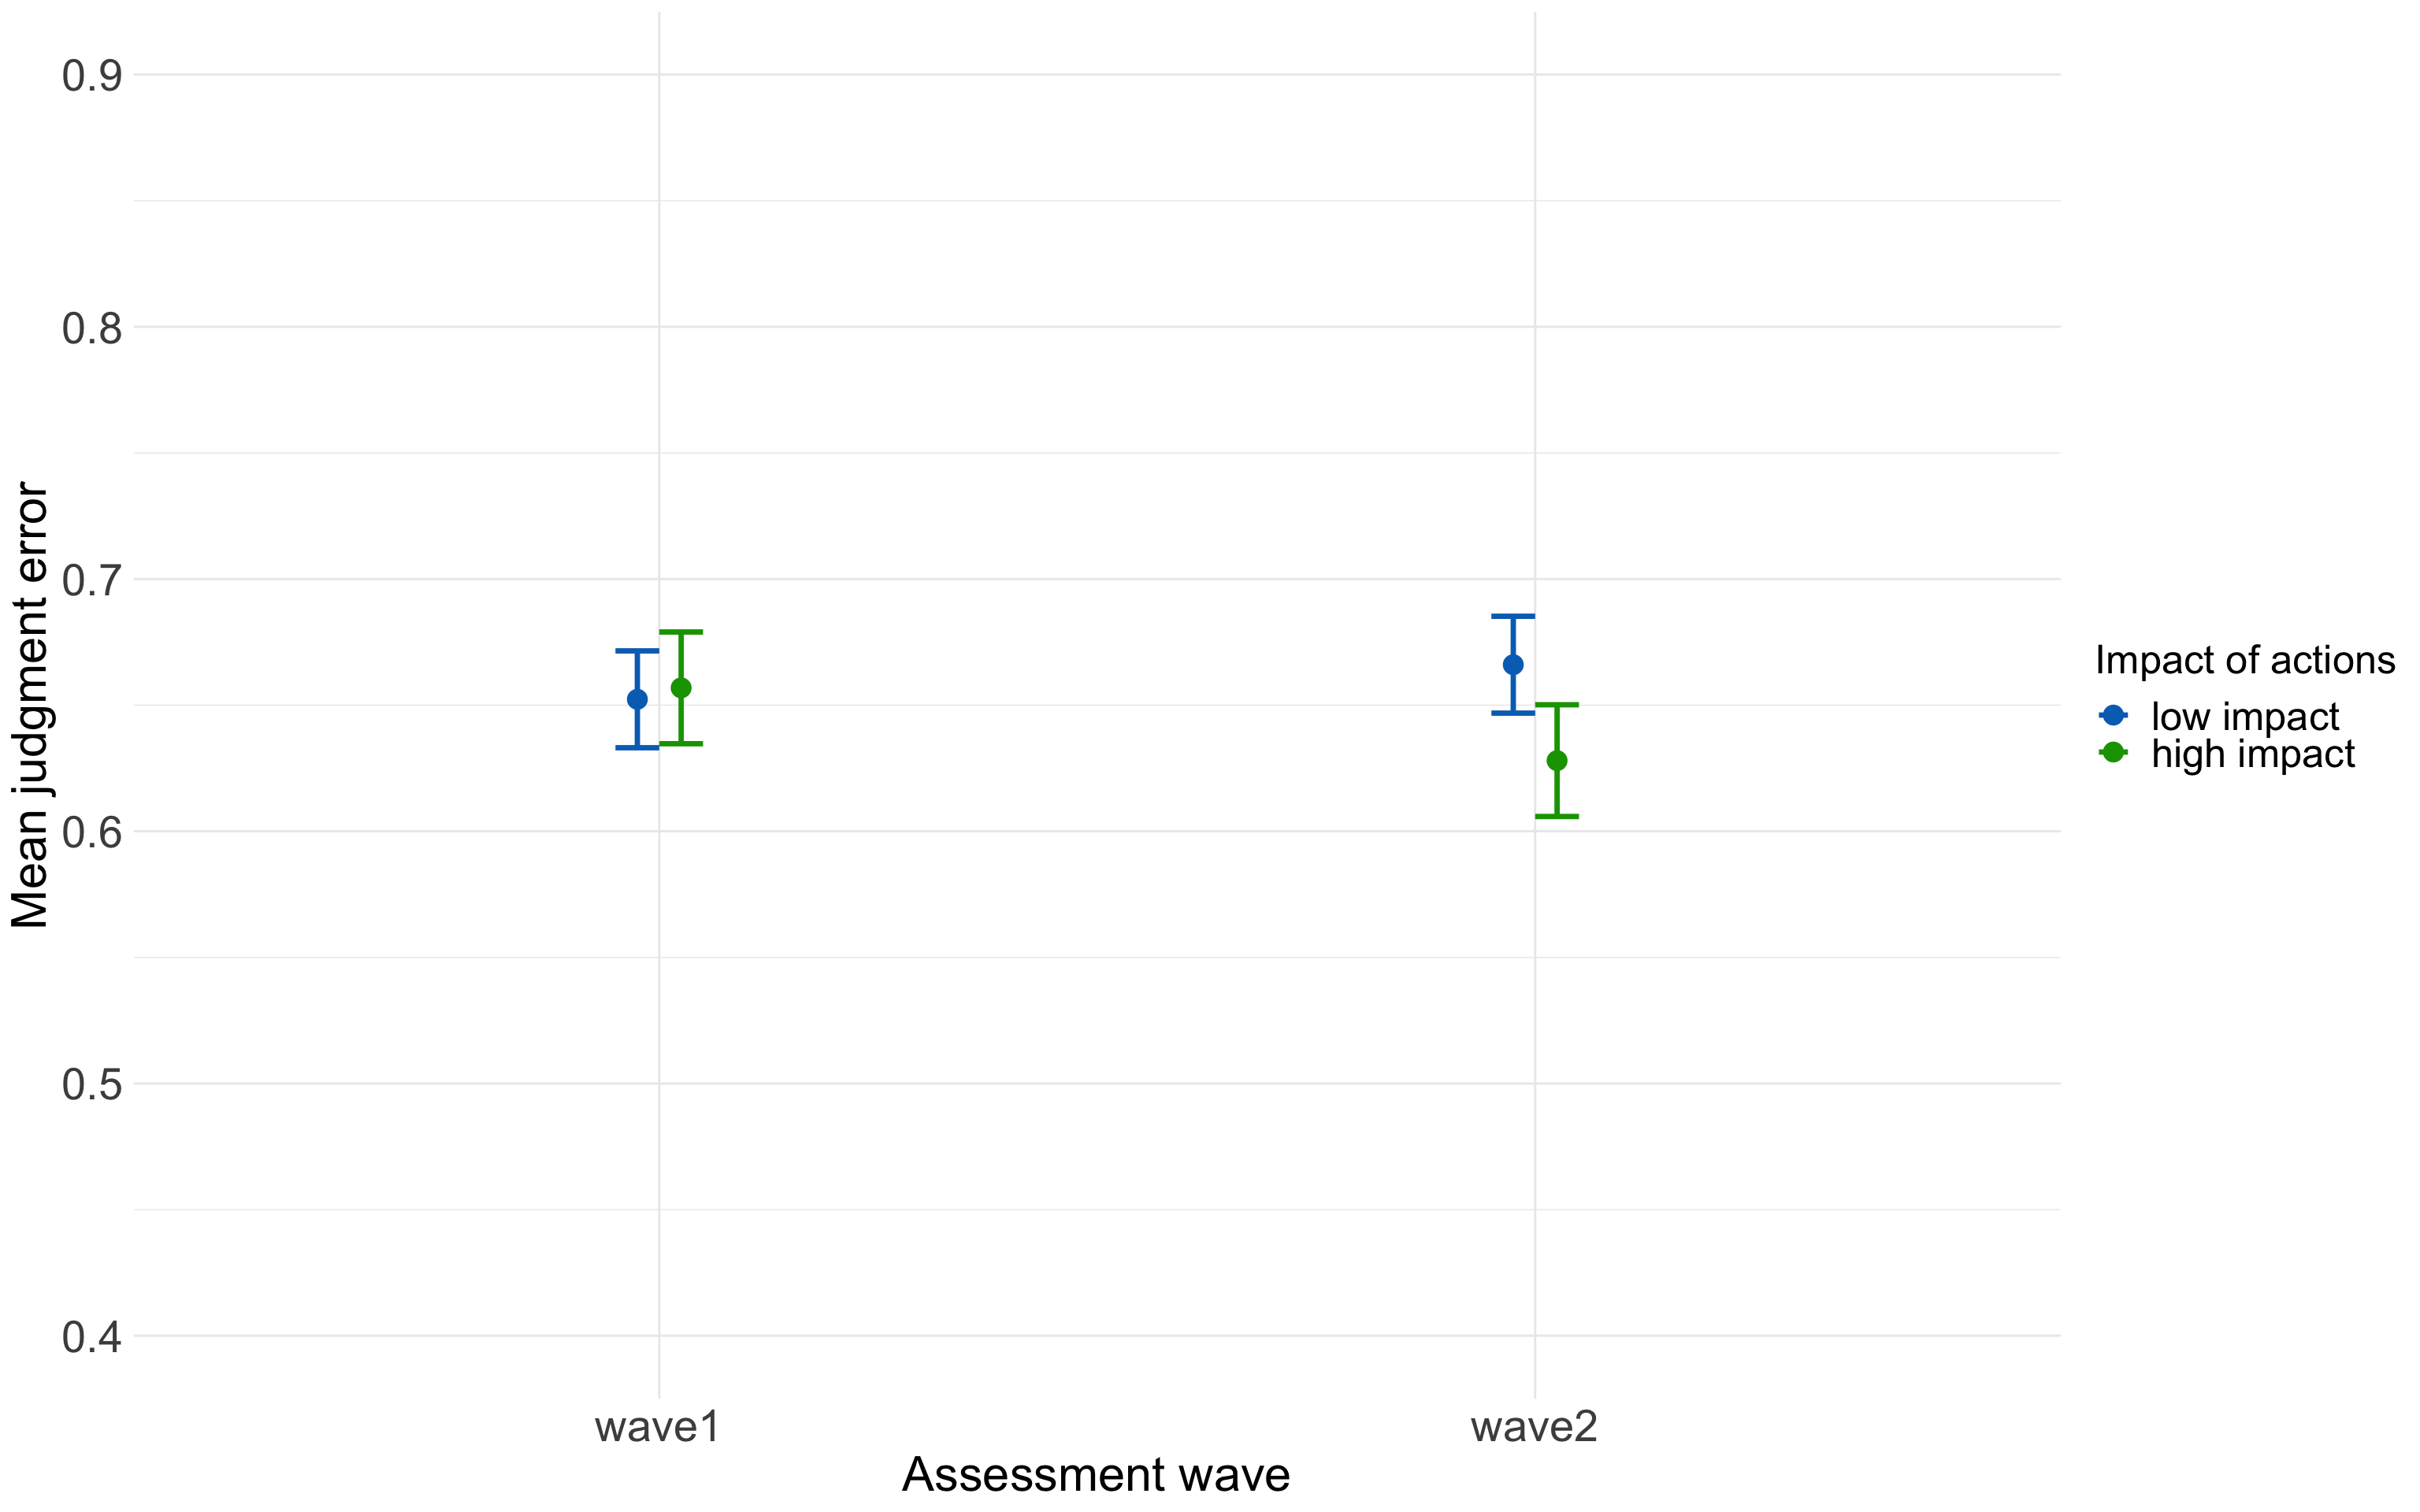
\includegraphics{analyses-judgment-new_files/figure-latex/unnamed-chunk-23-1} \end{center}

\hypertarget{plot-judgment-error-for-numeracy-across-waves}{%
\subsubsection{Plot: Judgment error for numeracy across
waves}\label{plot-judgment-error-for-numeracy-across-waves}}

\begin{center}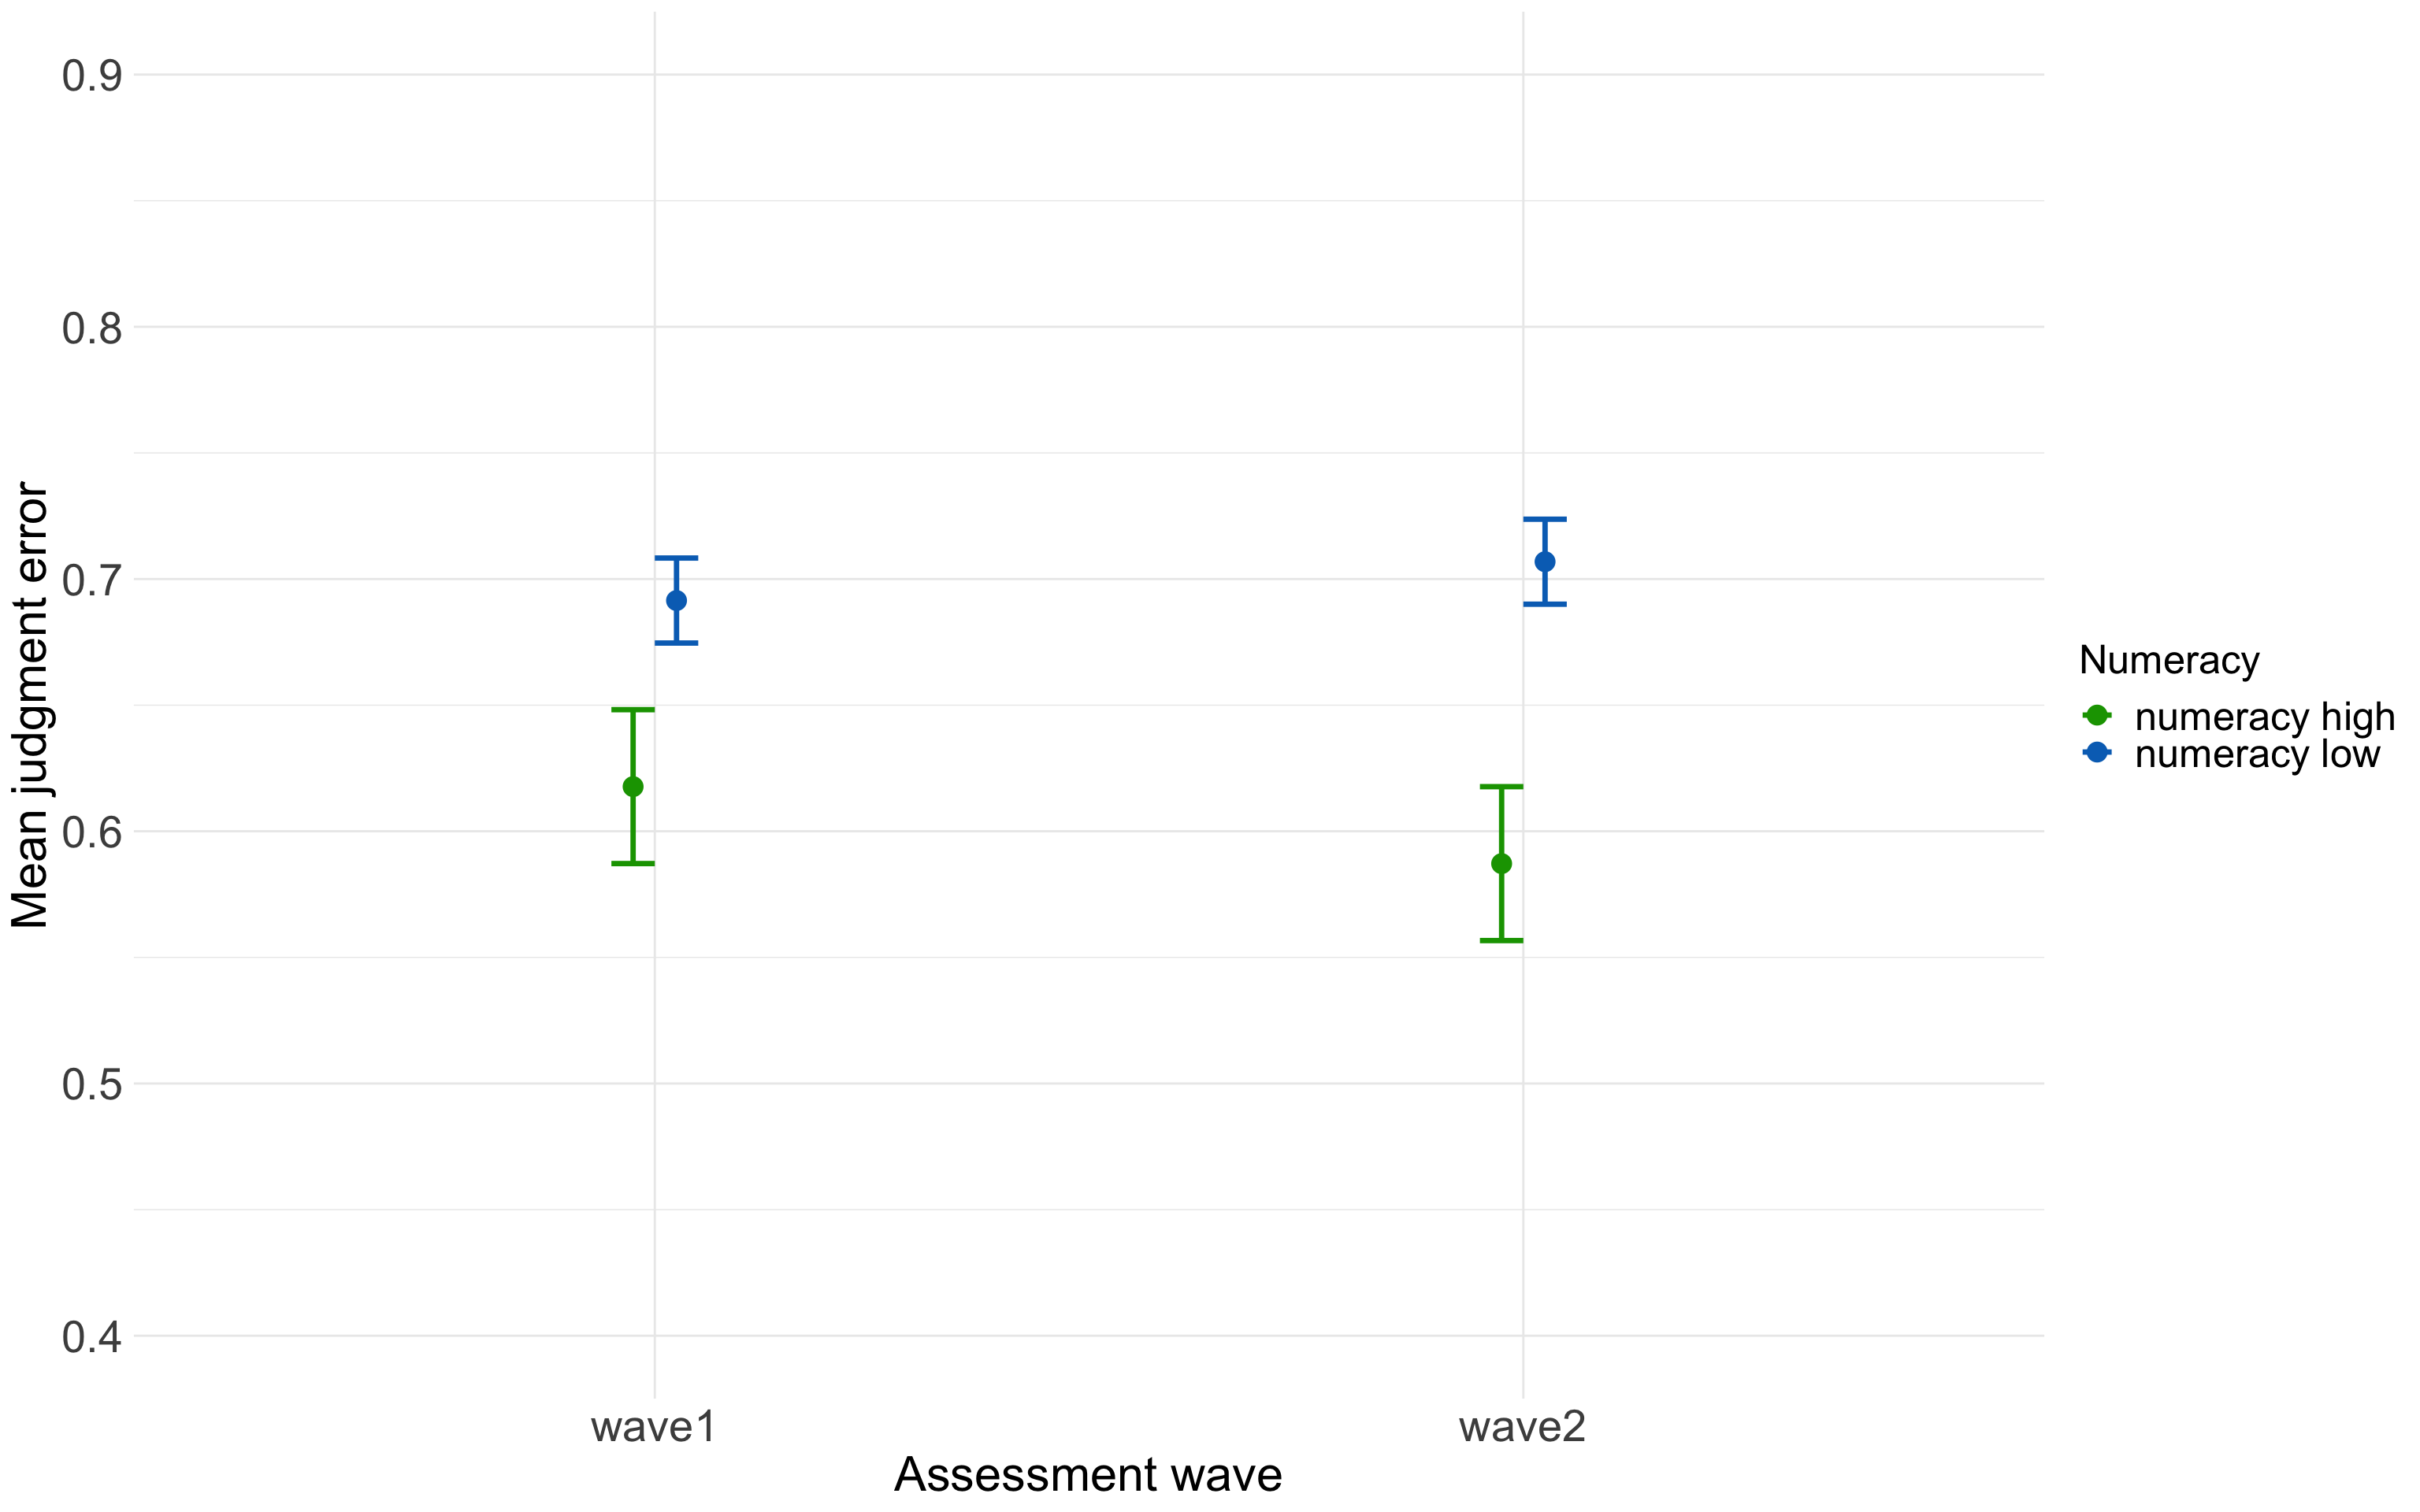
\includegraphics{analyses-judgment-new_files/figure-latex/unnamed-chunk-24-1} \end{center}

\hypertarget{plot-numeracy-by-wave-and-country}{%
\subsubsection{Plot: numeracy by wave and
country}\label{plot-numeracy-by-wave-and-country}}

\begin{center}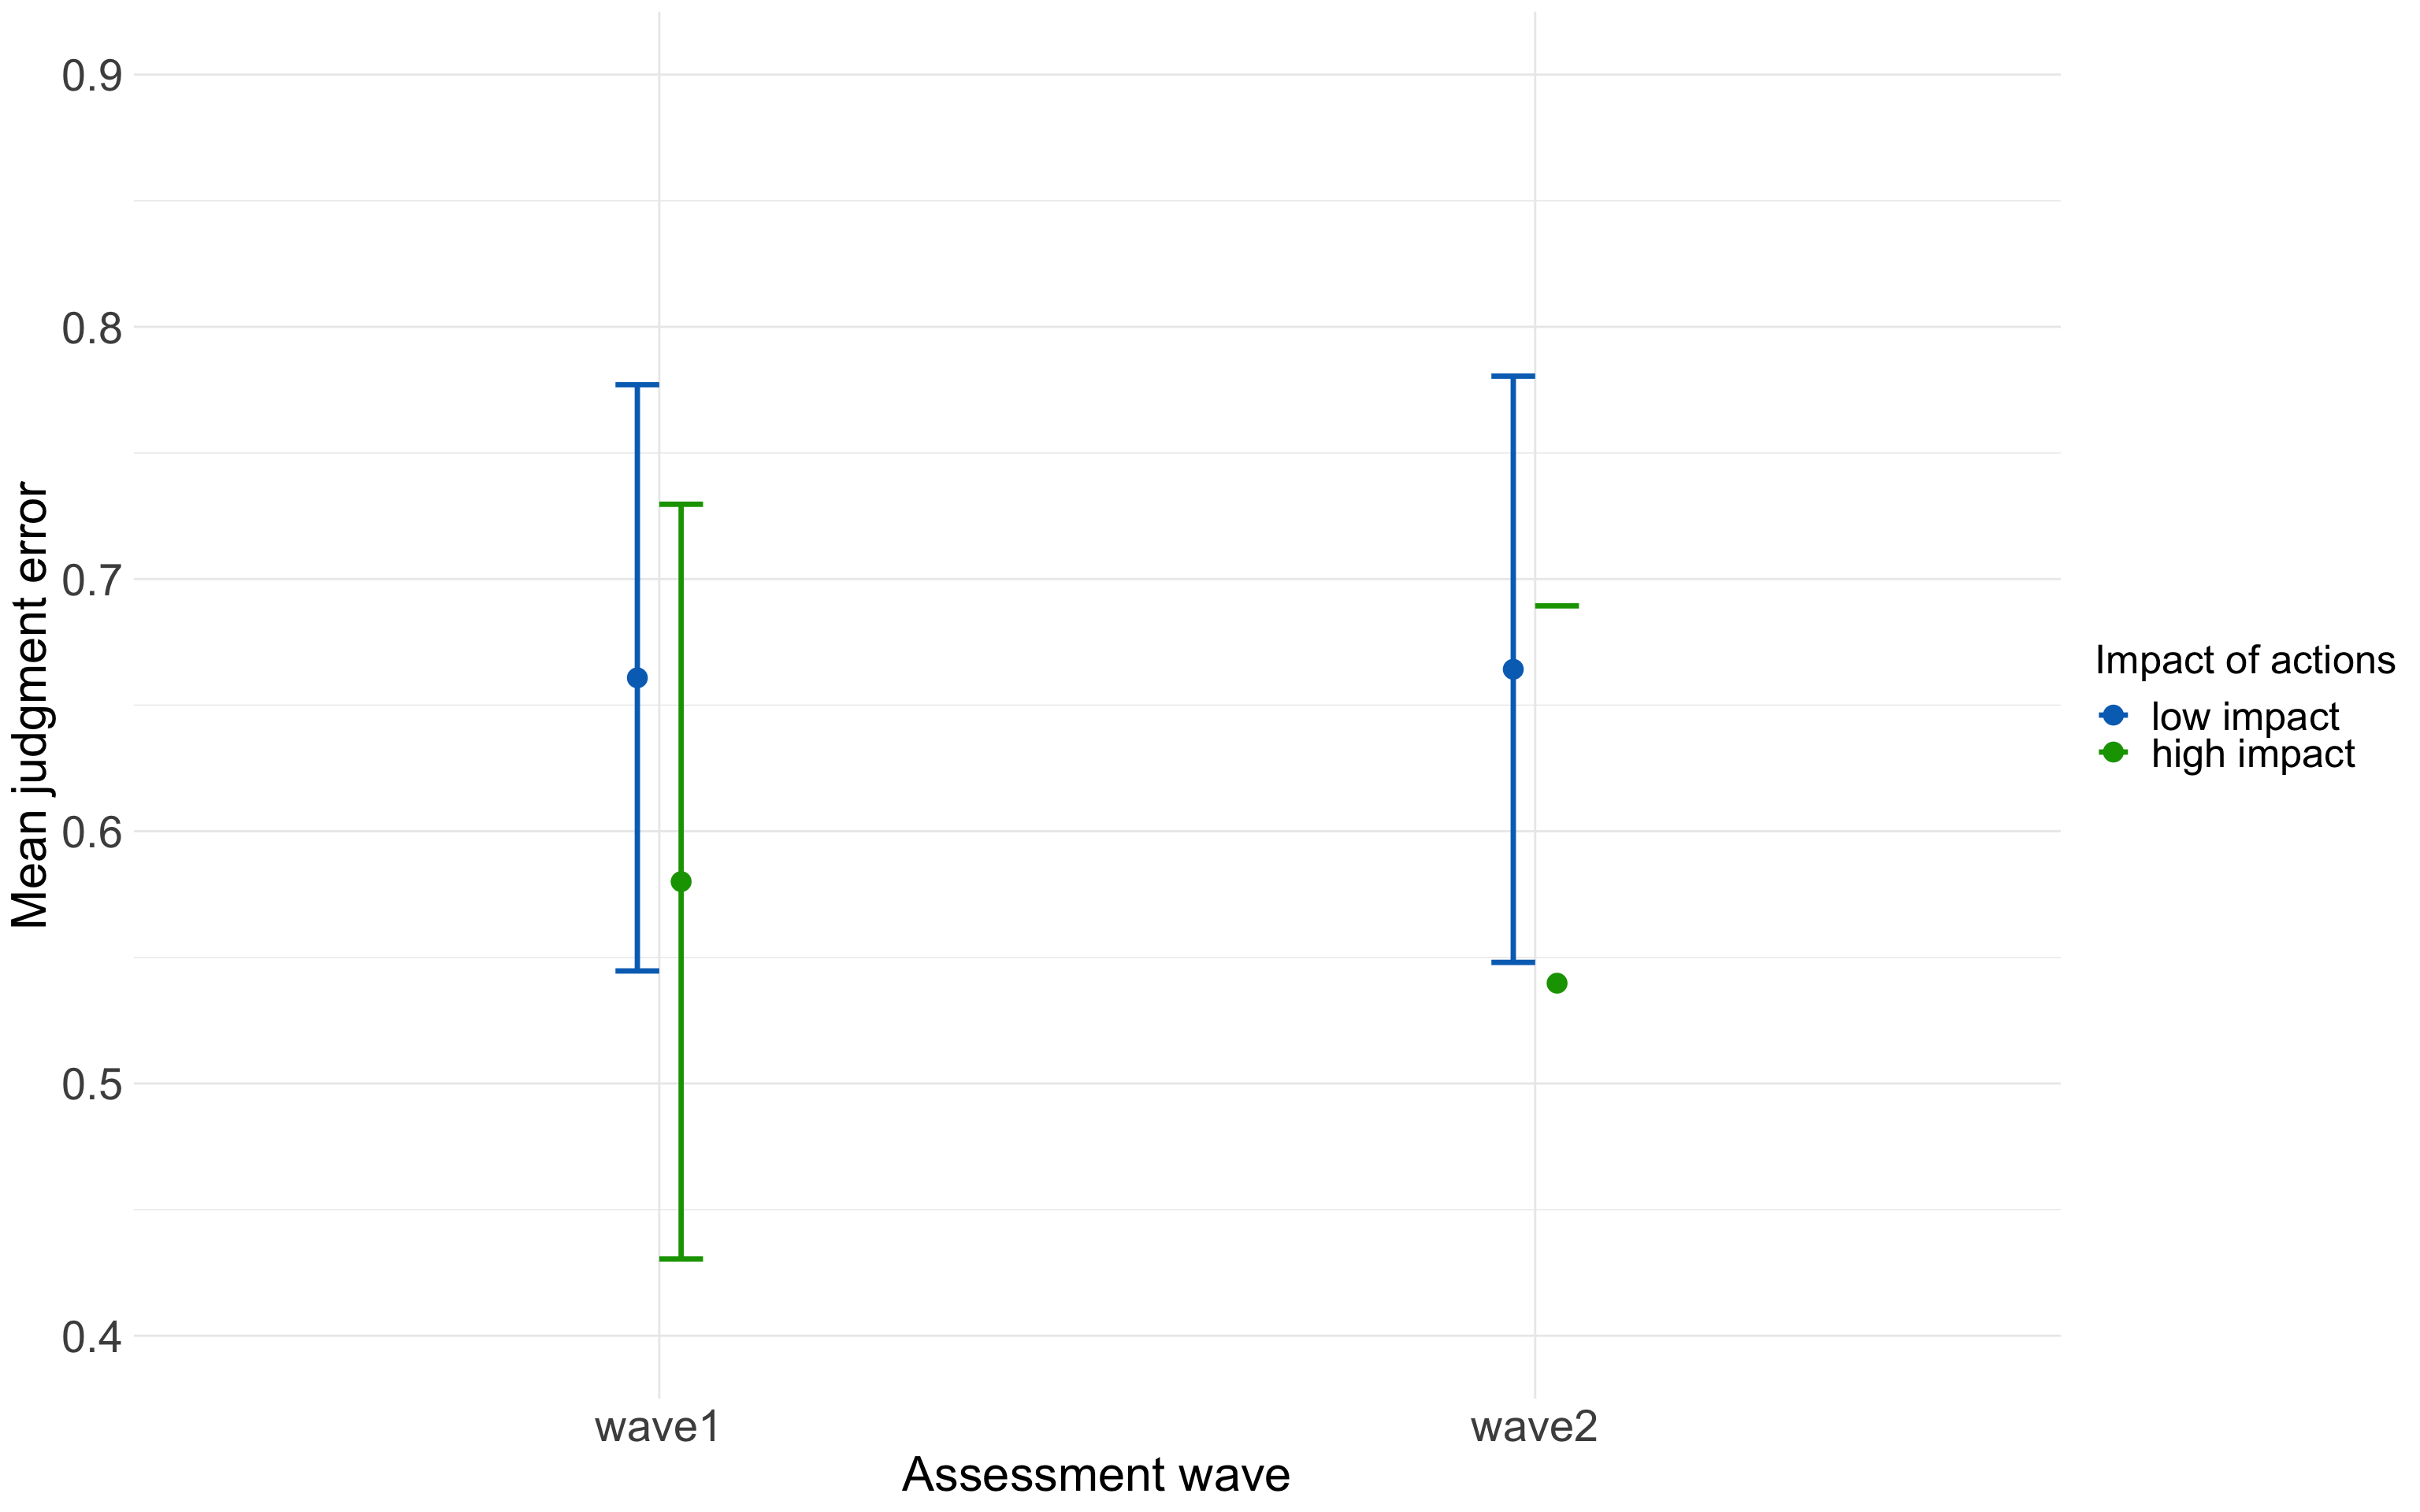
\includegraphics{analyses-judgment-new_files/figure-latex/unnamed-chunk-25-1} \end{center}

\hypertarget{plot-everything-in-one-plot}{%
\subsubsection{Plot: Everything in one
plot}\label{plot-everything-in-one-plot}}

\begin{center}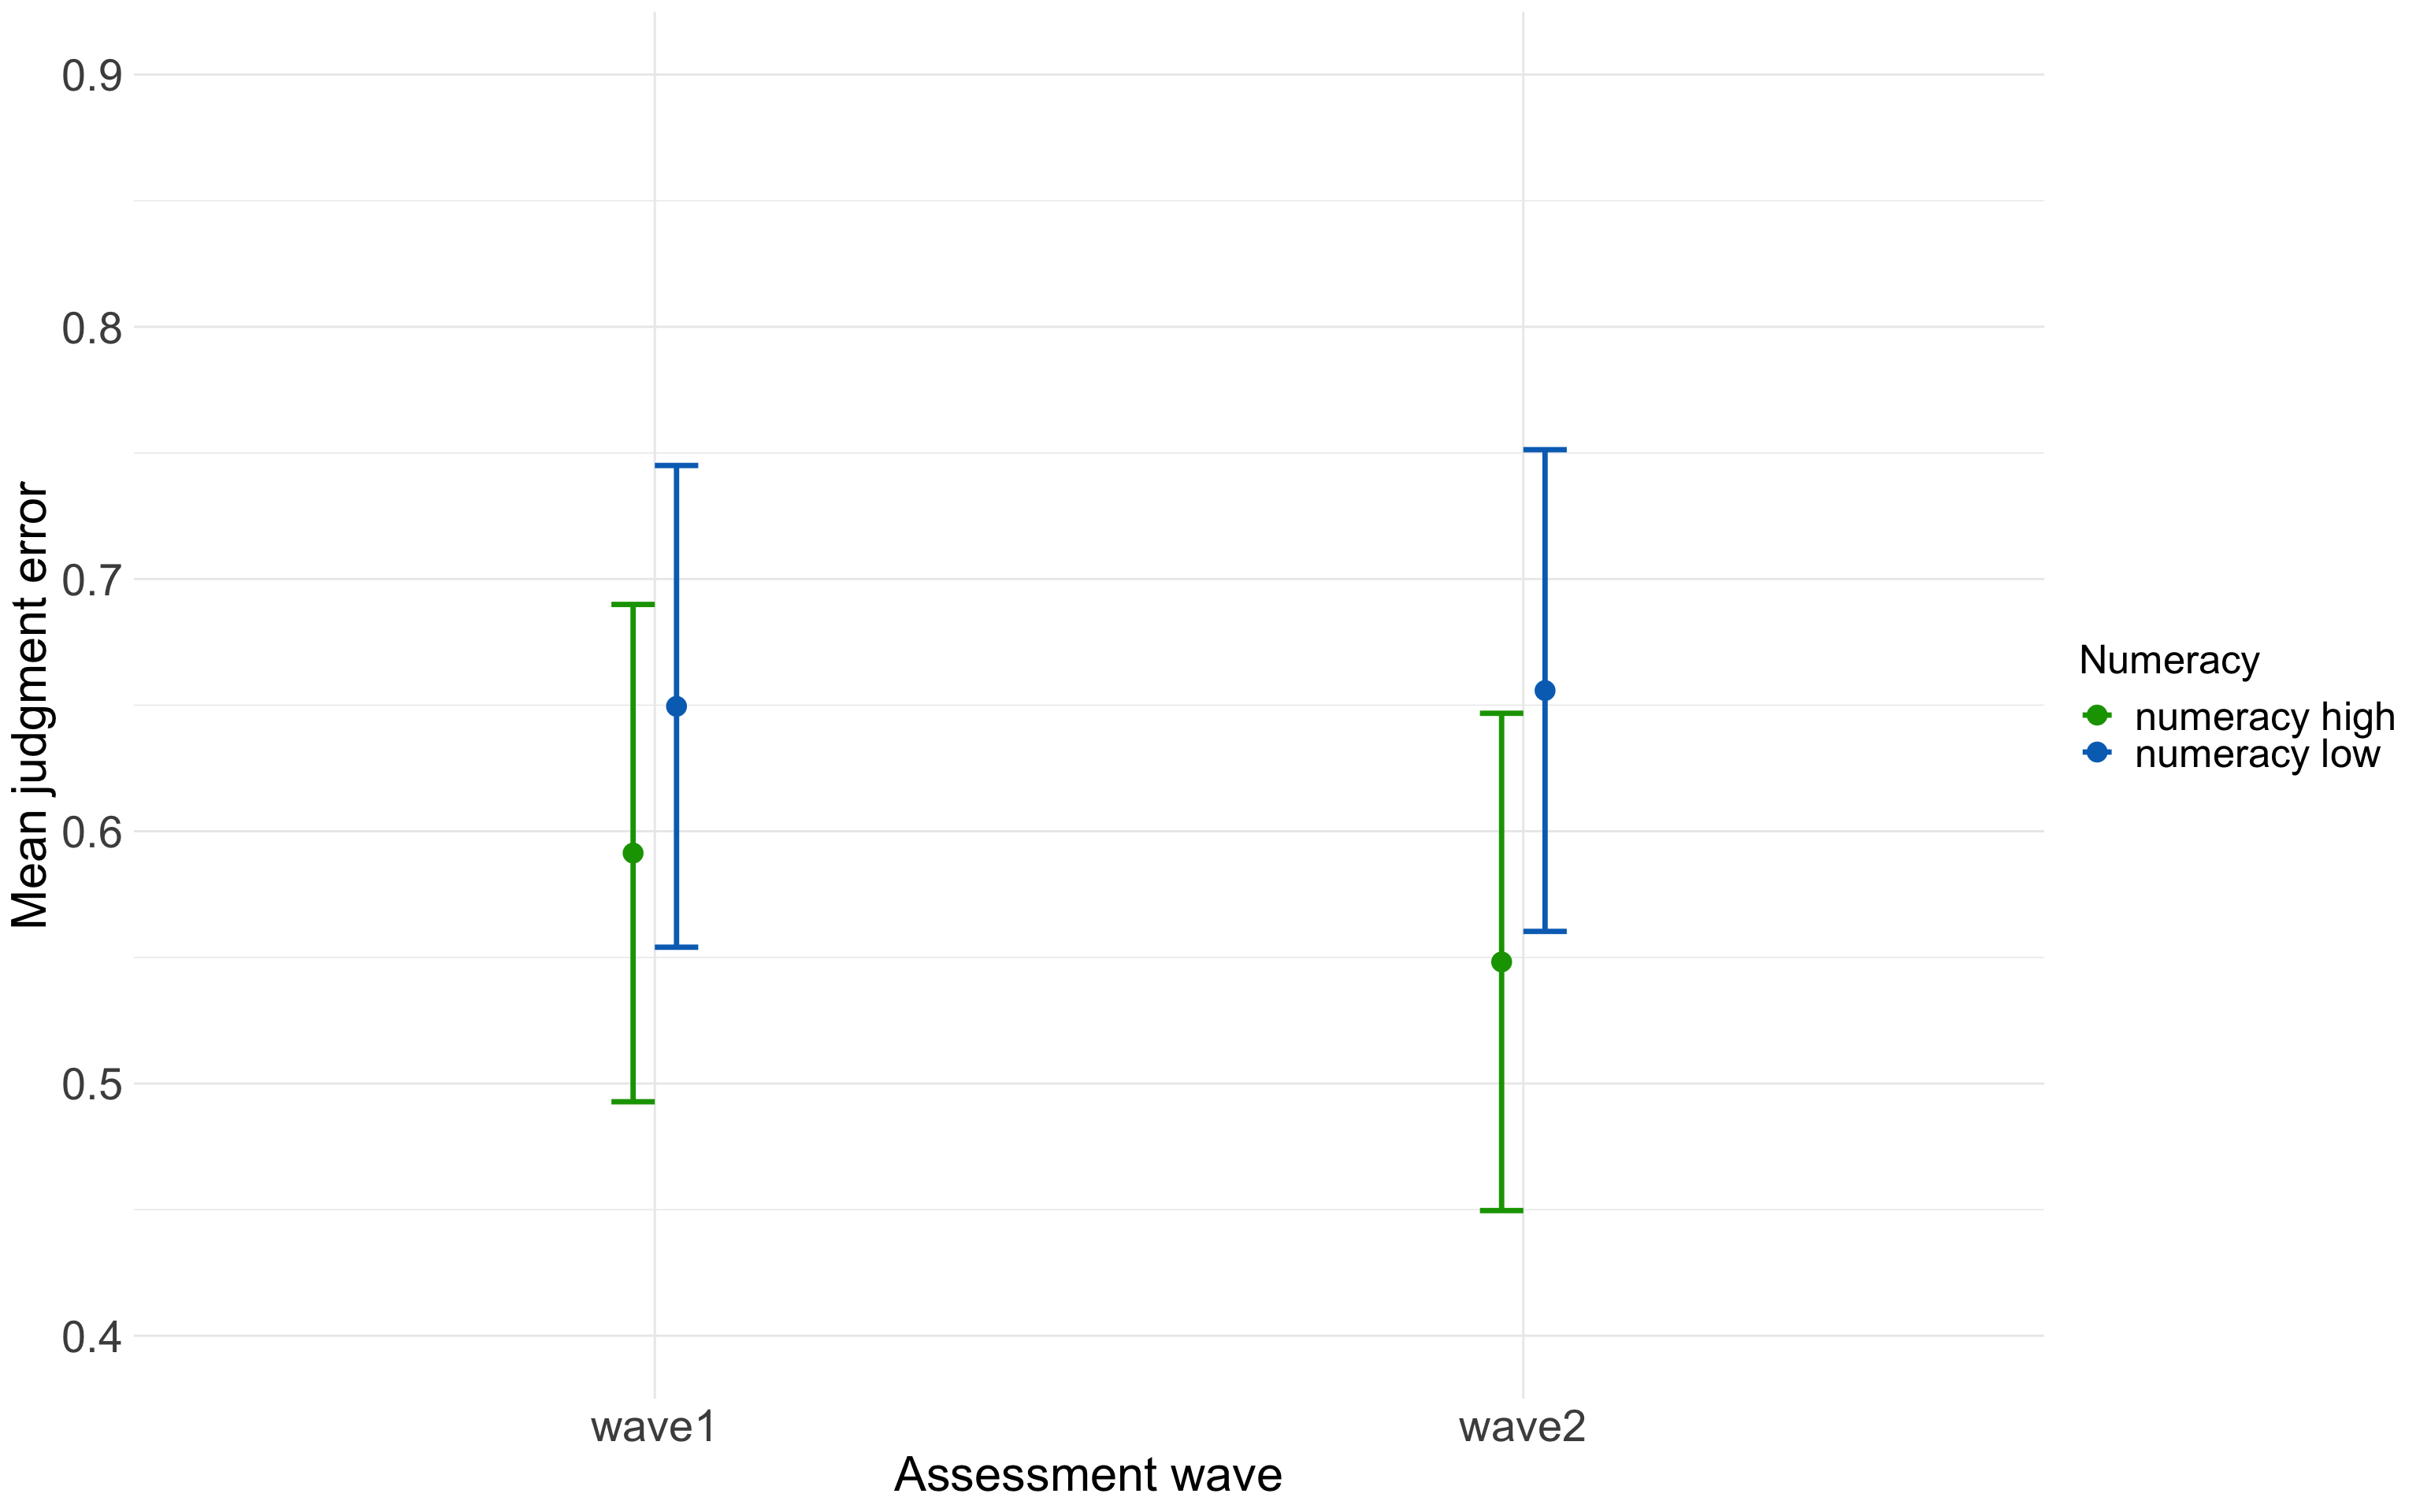
\includegraphics{analyses-judgment-new_files/figure-latex/unnamed-chunk-26-1} \end{center}

\hypertarget{plot-everything-in-one-plot2}{%
\subsubsection{Plot: Everything in one
plot2}\label{plot-everything-in-one-plot2}}

\begin{center}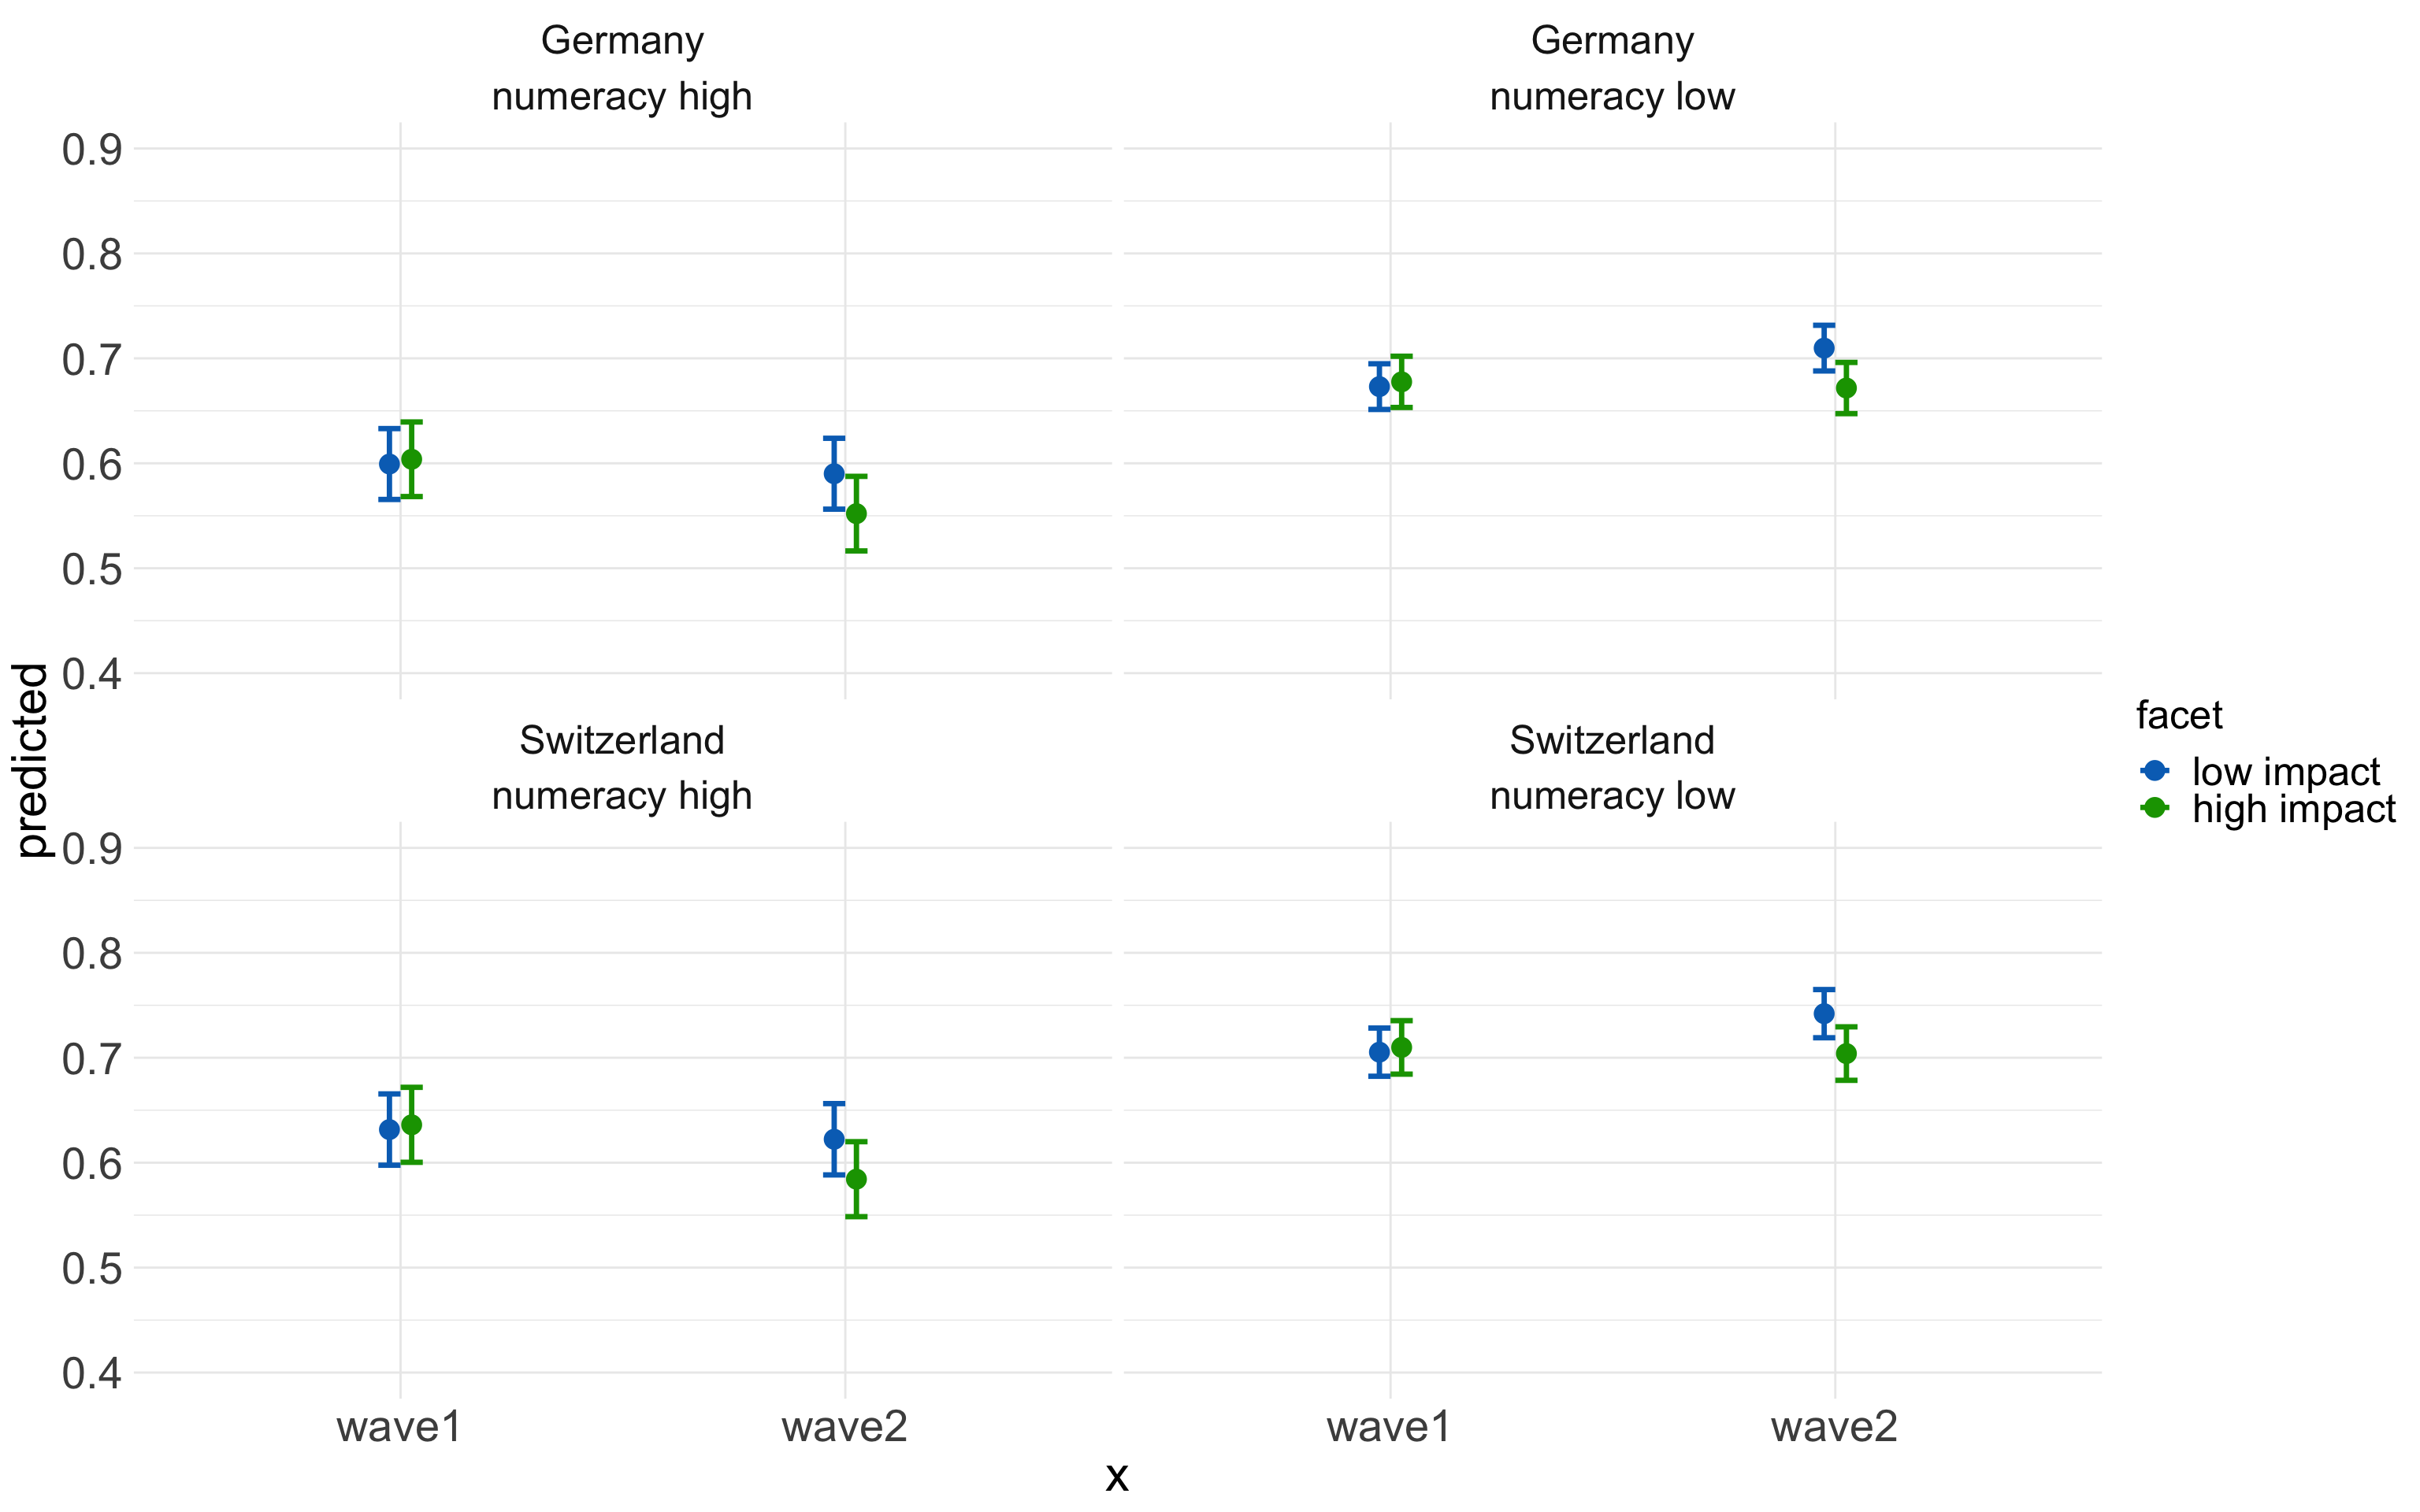
\includegraphics{analyses-judgment-new_files/figure-latex/unnamed-chunk-27-1} \end{center}

\hypertarget{by-country}{%
\subsection{By country}\label{by-country}}

\hypertarget{switzerland}{%
\subsubsection{Switzerland}\label{switzerland}}

\begin{verbatim}
## Analysis of Deviance Table (Type III Wald F tests with Kenward-Roger df)
## 
## Response: error
##                         F Df Df.res    Pr(>F)    
## (Intercept)     4372.6574  1  474.4 < 2.2e-16 ***
## numeracy.f        31.0434  1  453.0 4.336e-08 ***
## wave               0.4455  1 6821.0 0.5044796    
## impact            87.6079  1 6821.0 < 2.2e-16 ***
## numeracy.f:wave   10.9238  1 6821.0 0.0009543 ***
## wave:impact        3.0367  1 6821.0 0.0814473 .  
## ---
## Signif. codes:  0 '***' 0.001 '**' 0.01 '*' 0.05 '.' 0.1 ' ' 1
\end{verbatim}

\begin{verbatim}
## # Effect Size for ANOVA (Type III)
## 
## Parameter       | Eta2 (partial) |       95% CI
## -----------------------------------------------
## numeracy.f      |           0.06 | [0.03, 1.00]
## wave            |       6.53e-05 | [0.00, 1.00]
## impact          |           0.01 | [0.01, 1.00]
## numeracy.f:wave |       1.60e-03 | [0.00, 1.00]
## wave:impact     |       4.45e-04 | [0.00, 1.00]
## 
## - One-sided CIs: upper bound fixed at [1.00].
\end{verbatim}

~

error

Predictors

Estimates

CI

p

(Intercept)

0.65

0.63~--~0.67

\textless0.001

numeracy f1

-0.05

-0.07~--~-0.04

\textless0.001

wave1

0.00

-0.01~--~0.02

0.504

impact1

0.06

0.04~--~0.07

\textless0.001

numeracy f1 × wave1

0.02

0.01~--~0.04

0.001

wave1 × impact1

-0.01

-0.02~--~0.00

0.081

Random Effects

σ2

0.24

τ00 m

0.02

ICC

0.06

N m

455

Observations

7280

Marginal R2 / Conditional R2

0.021 / 0.084

\hypertarget{plot-switzerland}{%
\subsubsection{Plot Switzerland}\label{plot-switzerland}}

\begin{verbatim}
## Scale for y is already present.
## Adding another scale for y, which will replace the existing scale.
\end{verbatim}

\begin{center}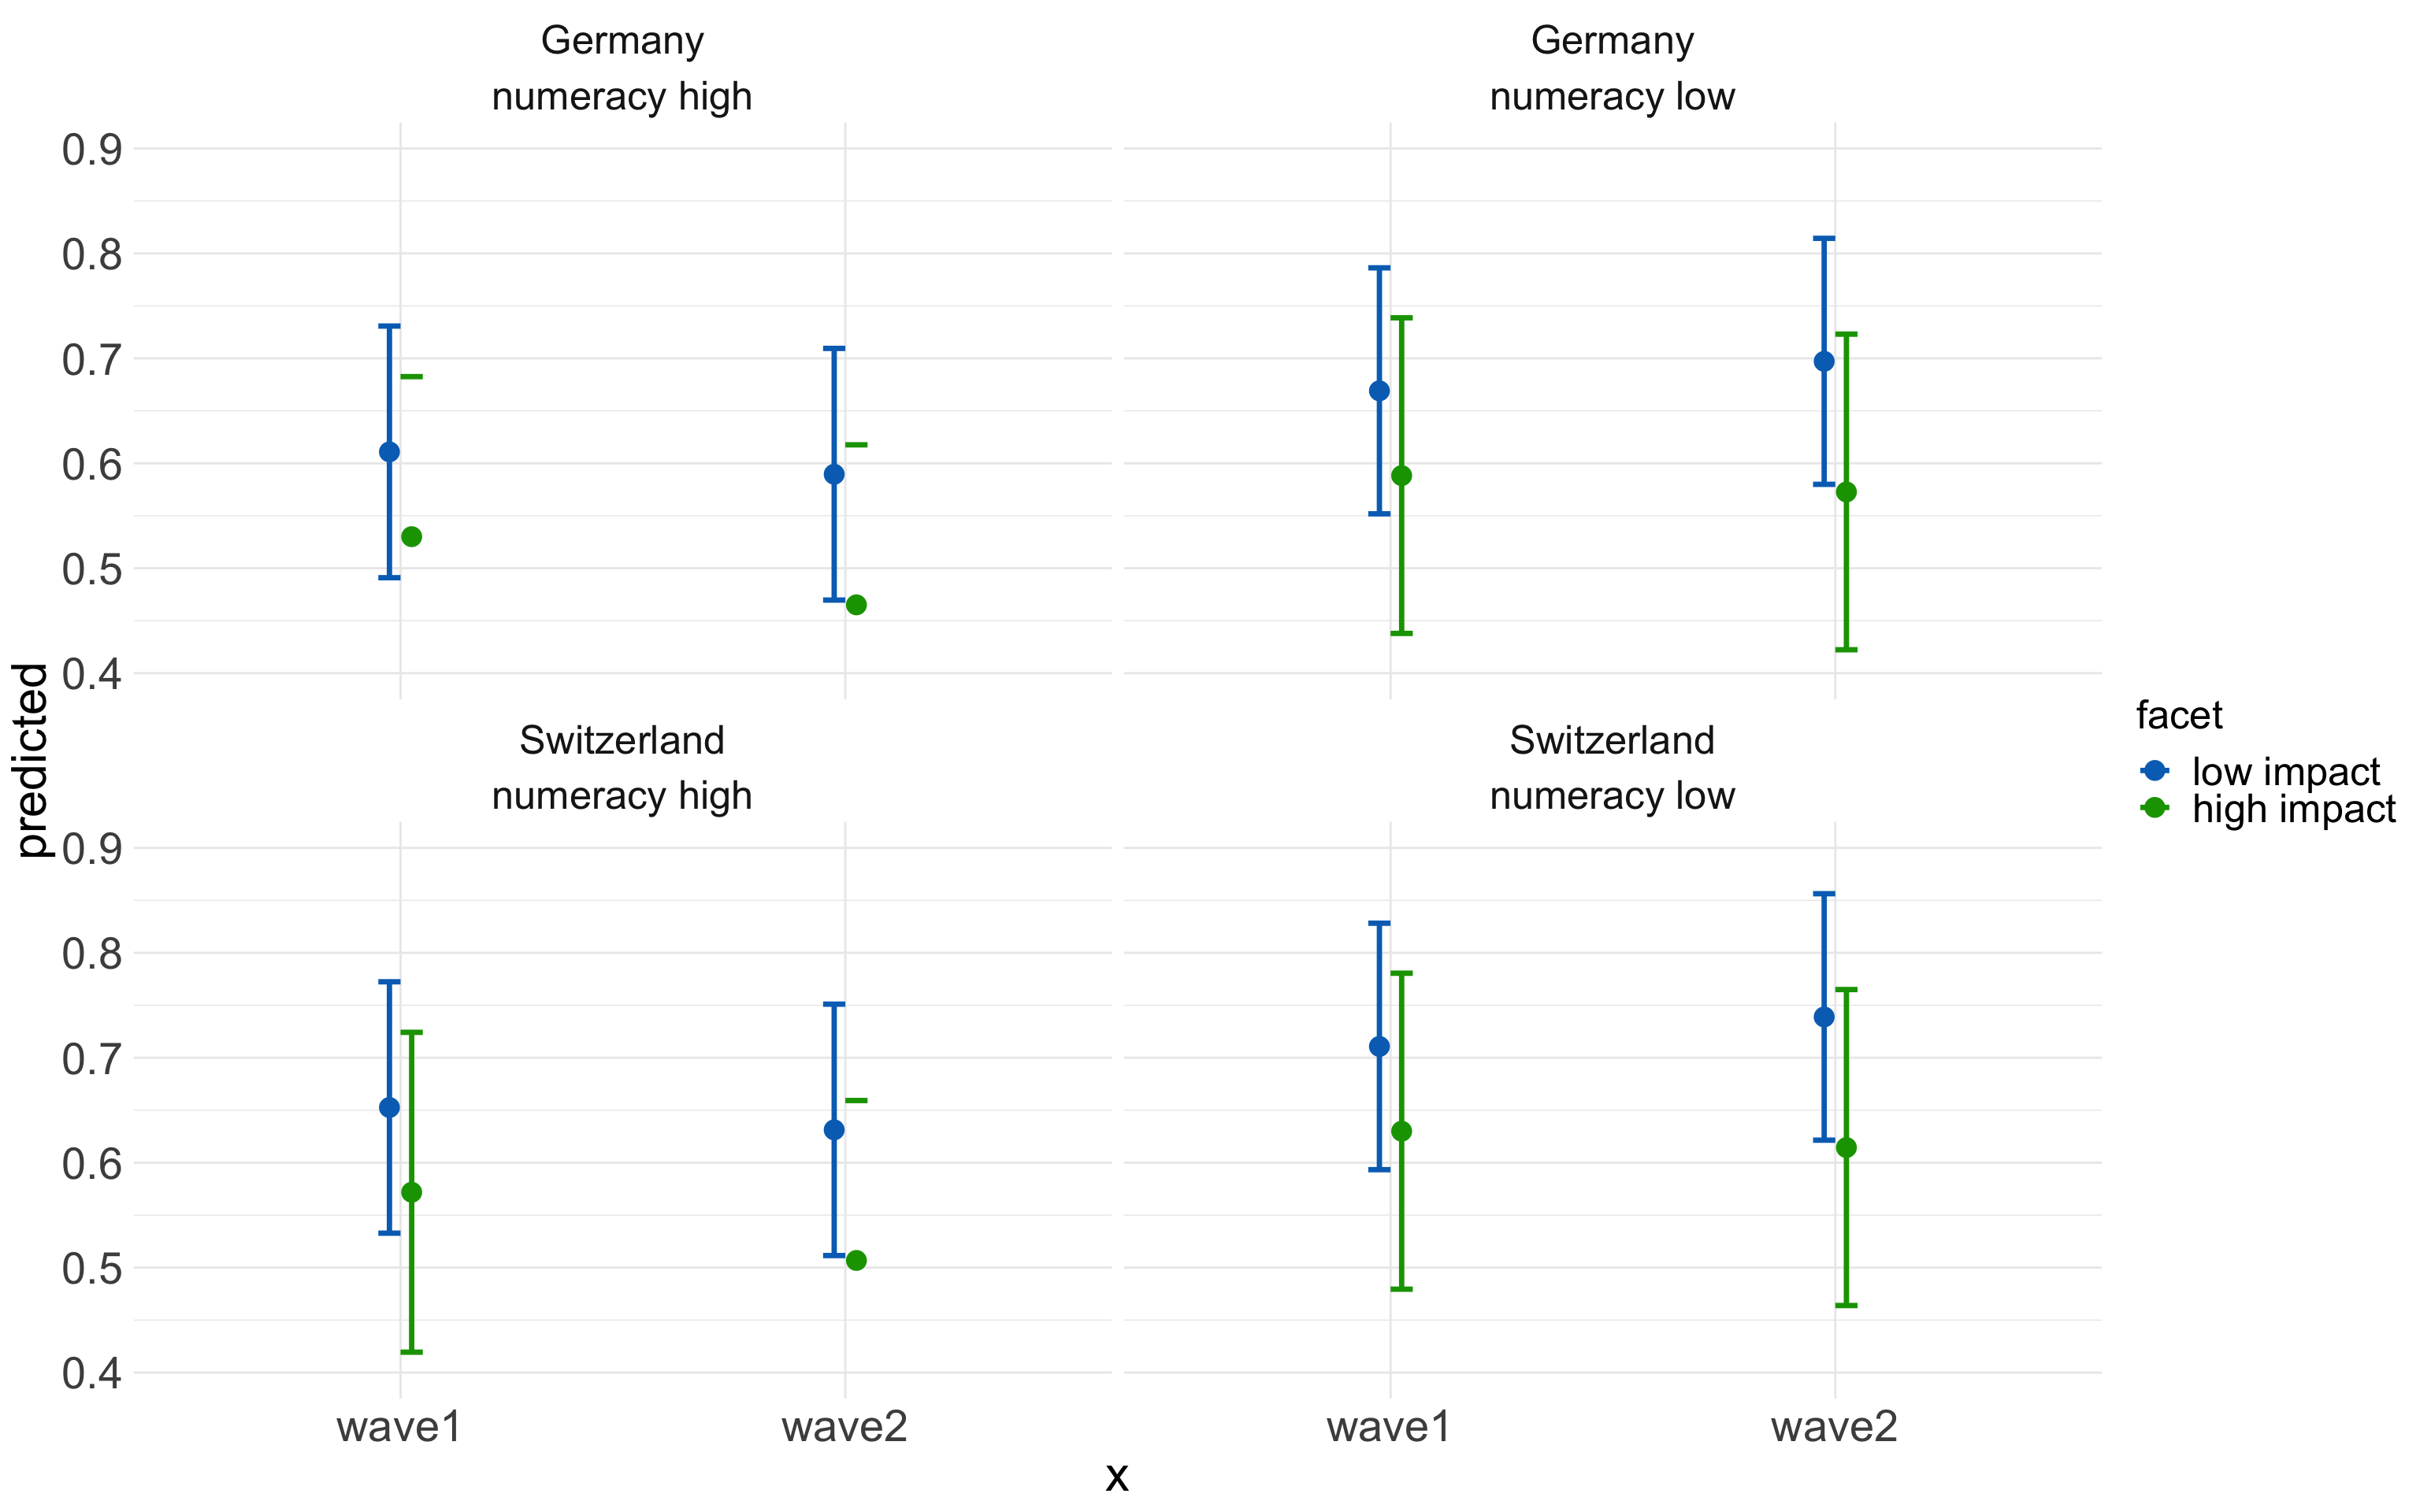
\includegraphics{analyses-judgment-new_files/figure-latex/unnamed-chunk-29-1} \end{center}

\hypertarget{germany}{%
\subsubsection{Germany}\label{germany}}

~

error

Predictors

Estimates

CI

p

(Intercept)

0.65

0.63~--~0.67

\textless0.001

numeracy f1

-0.04

-0.07~--~-0.02

\textless0.001

wave1

0.00

-0.01~--~0.01

0.704

impact1

-0.03

-0.04~--~-0.02

\textless0.001

numeracy f1 × wave1

0.00

-0.01~--~0.01

0.782

wave1 × impact1

-0.01

-0.02~--~-0.00

0.041

Random Effects

σ2

0.22

τ00 m

0.03

ICC

0.13

N m

525

Observations

8400

Marginal R2 / Conditional R2

0.009 / 0.135

\begin{verbatim}
## Analysis of Deviance Table (Type III Wald F tests with Kenward-Roger df)
## 
## Response: error
##                         F Df Df.res    Pr(>F)    
## (Intercept)     3218.1250  1  537.4 < 2.2e-16 ***
## numeracy.f        14.2630  1  523.0 0.0001772 ***
## wave               0.1445  1 7871.0 0.7038393    
## impact            38.0391  1 7871.0 7.276e-10 ***
## numeracy.f:wave    0.0766  1 7871.0 0.7819412    
## wave:impact        4.1912  1 7871.0 0.0406683 *  
## ---
## Signif. codes:  0 '***' 0.001 '**' 0.01 '*' 0.05 '.' 0.1 ' ' 1
\end{verbatim}

\begin{verbatim}
## # Effect Size for ANOVA (Type III)
## 
## Parameter       | Eta2 (partial) |       95% CI
## -----------------------------------------------
## numeracy.f      |           0.03 | [0.01, 1.00]
## wave            |       1.84e-05 | [0.00, 1.00]
## impact          |       4.81e-03 | [0.00, 1.00]
## numeracy.f:wave |       9.73e-06 | [0.00, 1.00]
## wave:impact     |       5.32e-04 | [0.00, 1.00]
## 
## - One-sided CIs: upper bound fixed at [1.00].
\end{verbatim}

\hypertarget{plot-germany}{%
\subsubsection{Plot Germany}\label{plot-germany}}

\begin{verbatim}
## Scale for y is already present.
## Adding another scale for y, which will replace the existing scale.
\end{verbatim}

\begin{center}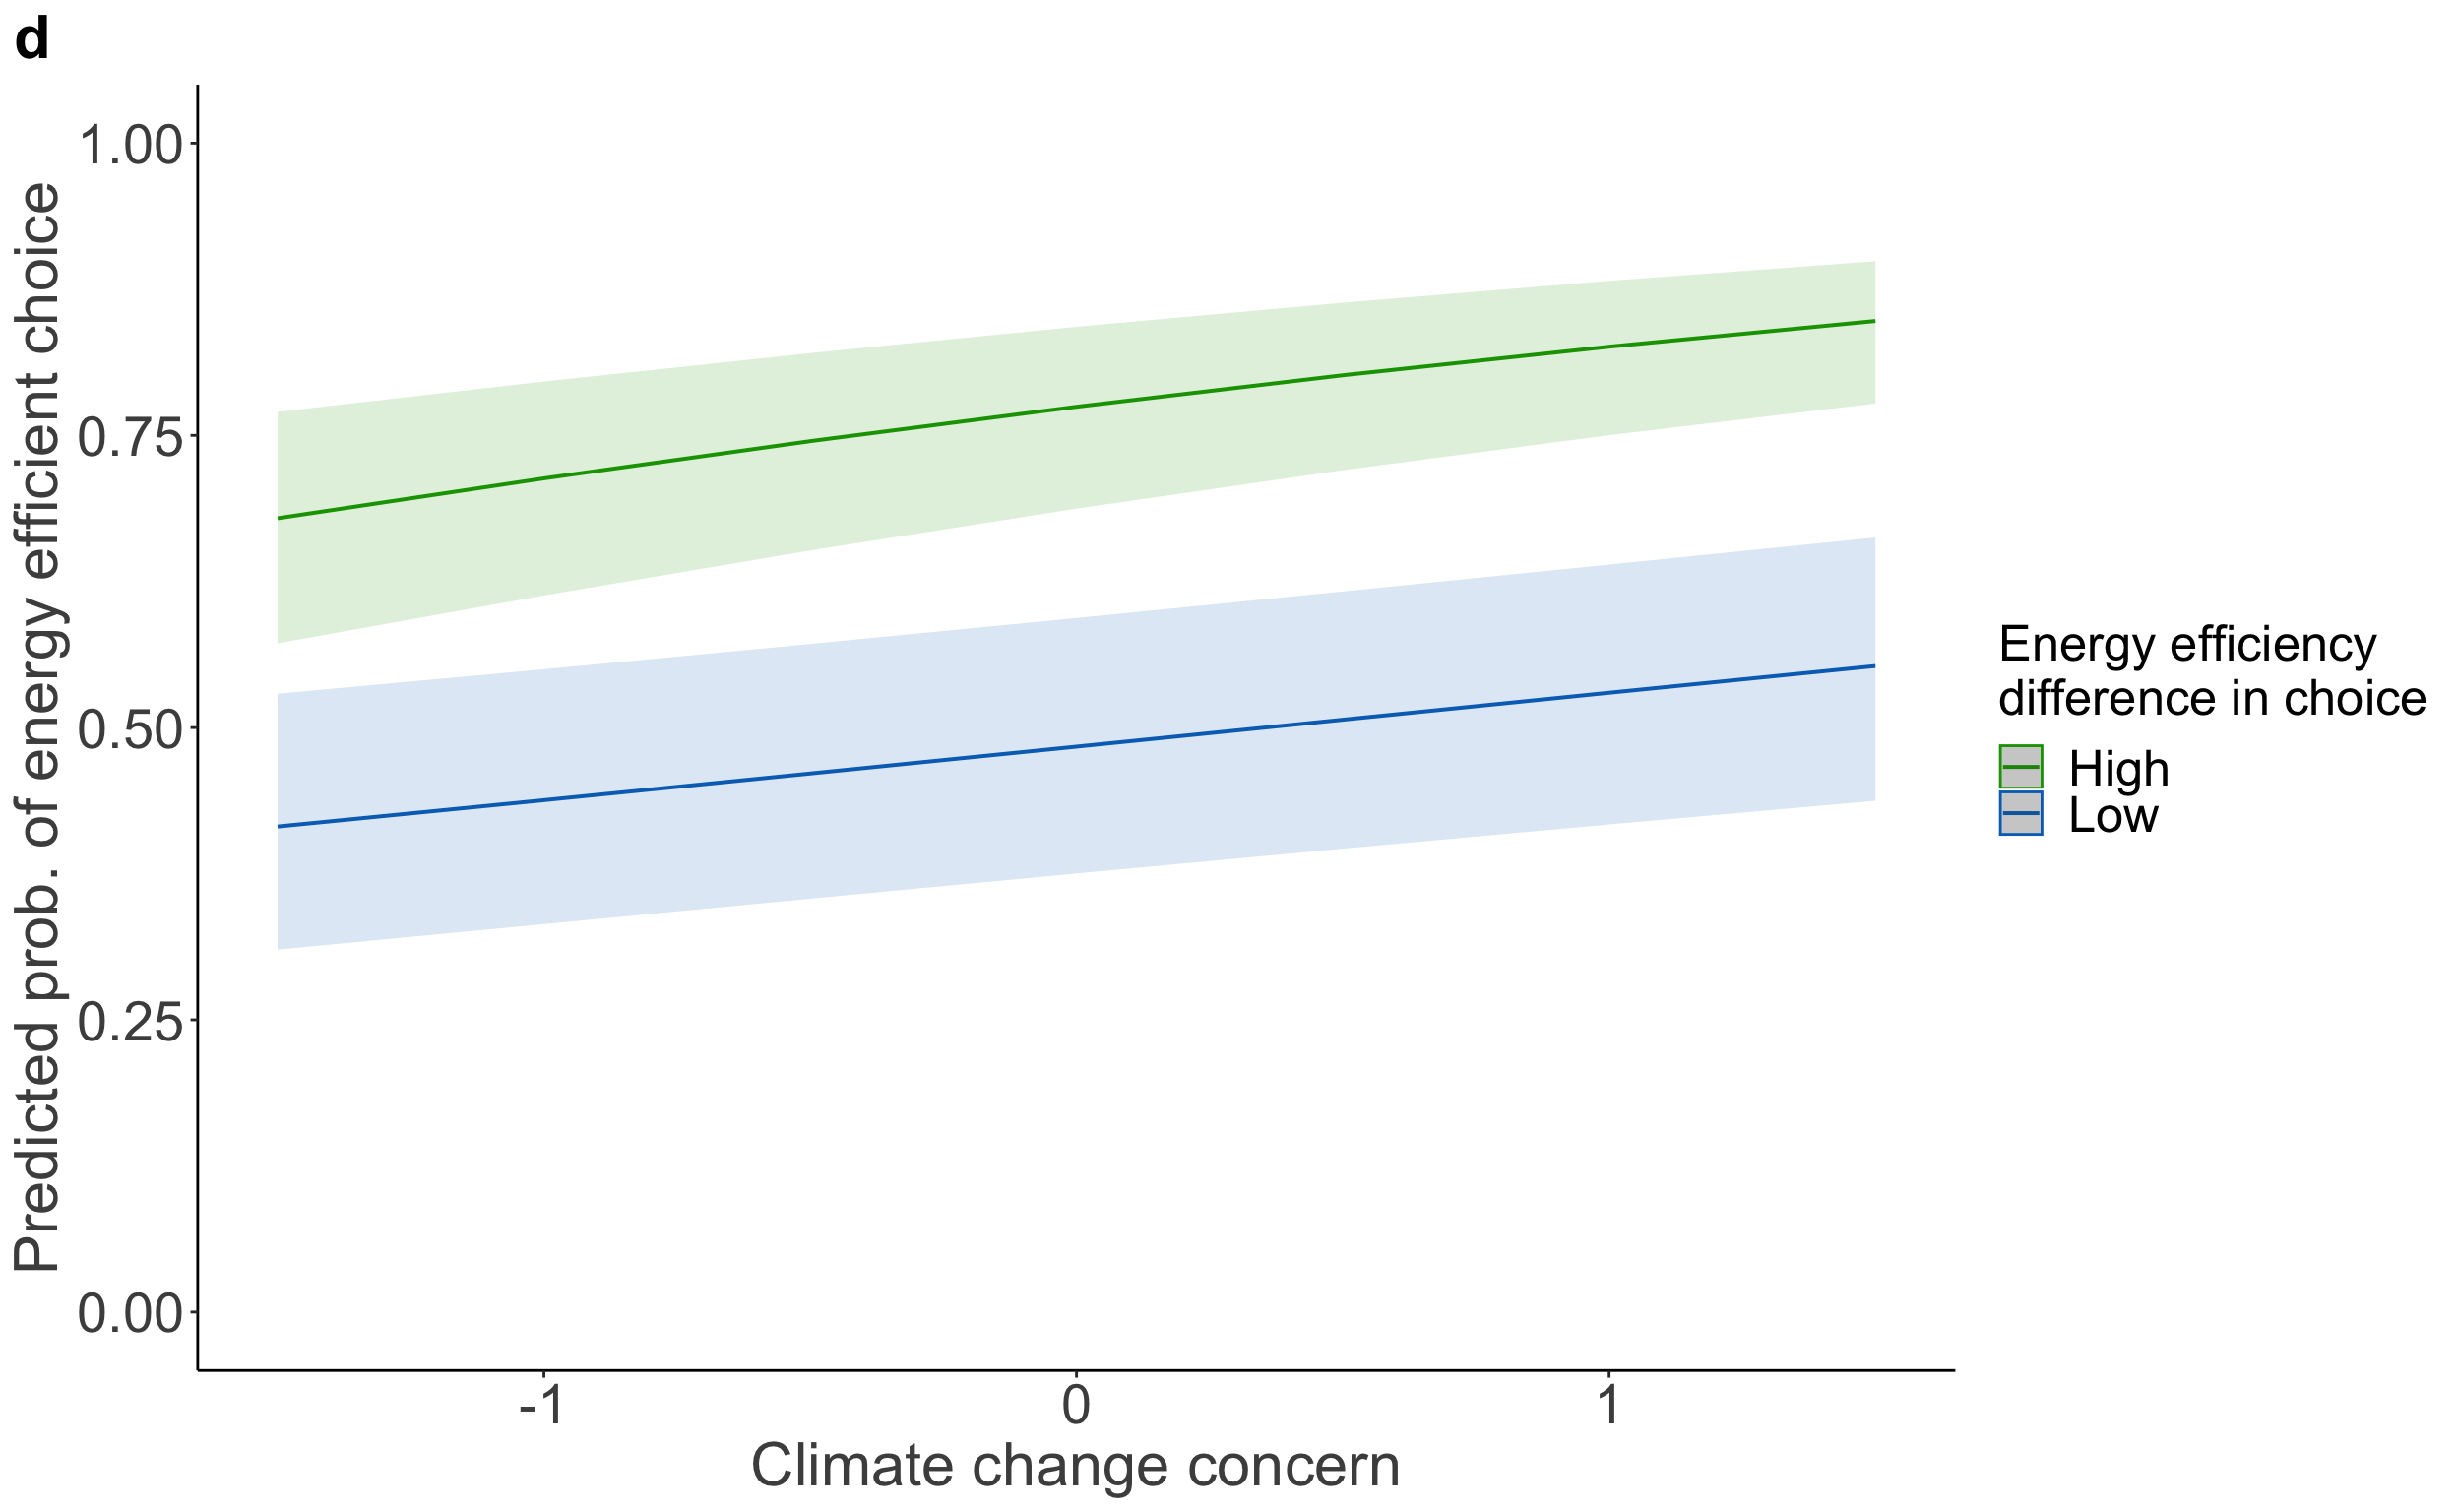
\includegraphics{analyses-judgment-new_files/figure-latex/unnamed-chunk-31-1} \end{center}

\hypertarget{across-waves-cohens-q}{%
\subsection{across waves cohens q}\label{across-waves-cohens-q}}

Original pre-registered plan to compare cohens q

For high numeracy people ths difference does approach a small effect
(such that the correlation between estimates and actual values ist
higher in wave2)

\begin{verbatim}
## Cohens q = -0.0491670467886844
\end{verbatim}

high numeracy

\begin{verbatim}
## Cohens q = -0.0932812950061401
\end{verbatim}

For high numeracy people the cohens q (rounded) can be categorized as a
small effect

without pattern people

\begin{verbatim}
## Cohens q = -0.0497625254424904
\end{verbatim}

high numeracy no pattern people

\begin{verbatim}
## Cohens q = -0.0912862921460136
\end{verbatim}

For high numeracy people the cohens q (rounded) can be categorized as a
small effect

\end{document}
